\documentclass[11pt,a4paper]{article}
\usepackage{fontspec}
\setmainfont{TeX Gyre Pagella}
\newfontfamily\headfont{Inter}[UprightFont=*-ExtraBold,BoldFont=*-ExtraBold,Extension=.otf,Path=/usr/share/fonts/opentype/inter/]
\usepackage[a4paper,margin=2.3cm]{geometry}
\usepackage{graphicx,booktabs,float,caption,array,xcolor,longtable}
\usepackage{xurl}
\usepackage[hidelinks]{hyperref}
\usepackage{titlesec}
\usepackage[round]{natbib}
\usepackage{setspace}
\setstretch{1.05}
\renewcommand{\topfraction}{0.9}
\renewcommand{\bottomfraction}{0.8}
\renewcommand{\textfraction}{0.1}
\renewcommand{\floatpagefraction}{0.75}
\setlength{\parindent}{0pt}
\setlength{\parskip}{0.55em}
\titleformat{\section}{\headfont\Large}{\thesection}{0.8em}{}
\titleformat{\subsection}{\headfont\large}{\thesubsection}{0.8em}{}
\captionsetup{font=small,labelfont=bf}
\urlstyle{same}
\hypersetup{pdftitle={The Shape of the Tour},pdfauthor={Tristan Hotham}}

\begin{document}
\begin{center}
{\Large\bfseries The Shape of the Tour\par}
\vspace{0.4em}
{\large Every stage of the Tour de France, 1903 to 2026, mapped from start to finish\par}
\vspace{1.2em}
{\large Tristan Hotham\par}
\vspace{0.3em}
{\small Independent researcher\\
ORCID: 0000-0003-4931-9349\\
DOI: https://doi.org/10.5281/zenodo.23873013\par}
\vspace{0.8em}
2026
\end{center}

\begin{quote}
\small
\begin{center}\textbf{Abstract}\end{center}
I geocode the start and finish towns of all 2,427 stages of the men's Tour de France from 1903 to 2026, and the 42 stages of the Tour de France Femmes since 2022, using Thomas Camminady's LeTourDataSet and the GeoNames cities1000 gazetteer. 95.8\% of the 4,938 starts and finishes are located, at 701 places; most of the rest are summit finishes and ski stations. Drawn as straight lines, the stages show how the race changed shape. In the 1920s, 92\% of French stage towns lay within 50 km of the coast or a land border, against 37\% of the country's area; in the 2020s the share is 49\%. Until the 1930s every stage began where the previous one ended; in the 2020s 88\% do not, and the gaps sum to about 1,152 km a Tour in straight lines. Paris (161 starts and finishes), Bordeaux (137) and Pau (133) are the most used stage towns, and every one of the 96 départements of metropolitan France has hosted at least one start or finish. 27 Tours started abroad, the first in 1954, and 14 of the 27 since 2000; 12.5\% of stages touched another country. The race shrank from 5,745 km in 1926 to 3,333 km in 2026 while the winner's average speed rose from 25.7 km/h in 1903 to 45.08 km/h. French riders won 36 of the 106 editions with a winner in the official record, which has none for 1999 to 2005.

\textbf{Keywords:} Tour de France; cycling; sport geography; historical GIS; geocoding; GeoNames; route maps; open data
\end{quote}

\section{Introduction}
The Tour de France is a race and a map. Since 1903 its organisers have drawn a new route each year, and the route has always carried meaning: the early Tours were a lap of the national territory, a circuit of the frontiers and coasts that was part sporting contest and part celebration of France itself. Later Tours started abroad, hopped by train and plane between regions, and finished at summit stations built for skiers. This paper puts every stage of every Tour on one map, using open data, to describe how the route has changed and what has stayed the same.

The source is LeTourDataSet \citep{ltd}, Thomas Camminady's compilation of the official historical pages of the Tour \citep{letour}. It lists each stage's start and finish towns, the stage winner and the jersey holders, each Tour's total distance, and each rider's final result. It does not say where the towns are, and it has no route or length for single stages. I match the town names to GeoNames \citep{geonames} and treat each stage as a straight line from start to finish. The accompanying interactive map is at \url{https://maps.tristanhotham.com/tour-de-france/}.

\section{Data}
\textbf{Stages.} LeTourDataSet (commit c377920) has 2,434 stage rows for the men's Tour, 1903 to 2026, and 42 for the Tour de France Femmes, 2022 to 2026. Four stages appear twice with different winners because the win was shared; I merge each into one stage with both winners. In 2022 the opening time trial in Copenhagen is repeated and followed by two rows whose start and finish are both ``Transfert''; I drop those 3 rows. That leaves 2,427 men's stages in 113 Tours, with no race in 1915 to 1918 and 1940 to 1946, including 41 prologues and 217 half stages, and 42 women's stages.

\textbf{Riders.} The rider file gives each edition's final classification. The overall winner is the rider ranked first; the winner's average speed is the Tour's total distance divided by the winner's time, for editions decided on time (1905 to 1912 were decided on points). The file has no nationality, so I added the nationality of each of the 64 overall winners by hand and checked it against the team column for the 25 winners from years raced by national teams, where the team is a nation.

\textbf{Places.} GeoNames cities1000 lists 171,737 places with at least 1,000 inhabitants, with coordinates, country and administrative codes; I use the packaging by lutangar/cities.json (commit e5e759c). For France the second administrative code is the département. Country and département outlines are from Natural Earth \citep{naturalearth}.

\section{Methods}
\subsection{Geocoding}
I search only the 44,258 places in the thirteen countries the Tour has visited. Names are compared after removing accents, case, hyphens and apostrophes, with St and Ste spelt out; a stage name without an article may match a gazetteer name with one (Bourg-d'Oisans to Le Bourg-d'Oisans), but not the reverse. A hand-made table of 150 names covers four kinds of case: French names of foreign towns (Londres, Gand, Bâle, Saint-Sébastien); variants and short forms (Luchon for Bagnères-de-Luchon, Les Sables for Les Sables-d'Olonne); districts and venues inside one commune (Paris Champs-Élysées, Futuroscope at Chasseneuil-du-Poitou, Malo-les-Bains in Dunkirk); and ski stations named after their village (Alpe d'Huez to Huez, Saint-Lary-Soulan Col du Portet to Saint-Lary-Soulan). Summits and passes with no village in their name, such as the Puy de Dôme and Mont Ventoux, are deliberately left unmatched, as are lakes and venues spread over several communes and two regions.

When a name fits several places I keep an exact spelling match if there is one, and otherwise the candidate nearest the stage's other end; if that end is itself ambiguous, the candidate with the smallest mean distance to up to two unambiguous towns before and after it in race order. A French candidate within 400 km of that context is preferred, so that Belfort is the French town and not a district of Maastricht. The source uses ``Fribourg'' both for Fribourg in Switzerland and for Freiburg im Breisgau in Germany; both are offered and the nearer is kept. 343 starts and finishes were settled this way. Two checks found and corrected wrong namesakes: stages whose straight line was implausibly long, and jumps between one finish and the next start of more than 350 km. Every French place's département comes from its GeoNames code; in 8 cases on coasts and borders the code and the 1:10m polygon disagree, and the code is used.

\subsection{Measures}
A stage's line runs from its start town to its finish town. It is a lower bound on the distance ridden and says nothing about the road. A transfer is a stage that starts in a different place from the previous finish, measured the same way. A stage is abroad if either end lies outside France (Monaco and Andorra included) and crosses a border if its two ends are in different countries. A French stage town is near the edge if it lies within 50 km of the outline of metropolitan France, coast or land border, measured in the Lambert 93 projection; for comparison, 37.3\% of the area of metropolitan France lies that close to its edge. Each start and each finish counts once, so a town that hosts a finish and the next day's start counts twice.

\section{Results}
\subsection{Coverage}
4,731 of the 4,938 starts and finishes (95.8\%) and 766 of 863 distinct names are located, at 701 places. Both ends are located for 2,274 stages (92.1\%). Of the 207 unlocated starts and finishes, 75 are summits and passes, 66 ski stations, 50 villages missing from the gazetteer and 14 venues; 91\% of the unlocated summits and ski stations date from 1970 or later. The most frequent are the Puy de Dôme (15) and Mont Ventoux (13). Mountain finishes are therefore under-represented on the map, especially in recent decades.

\begin{figure}[tbp]\centering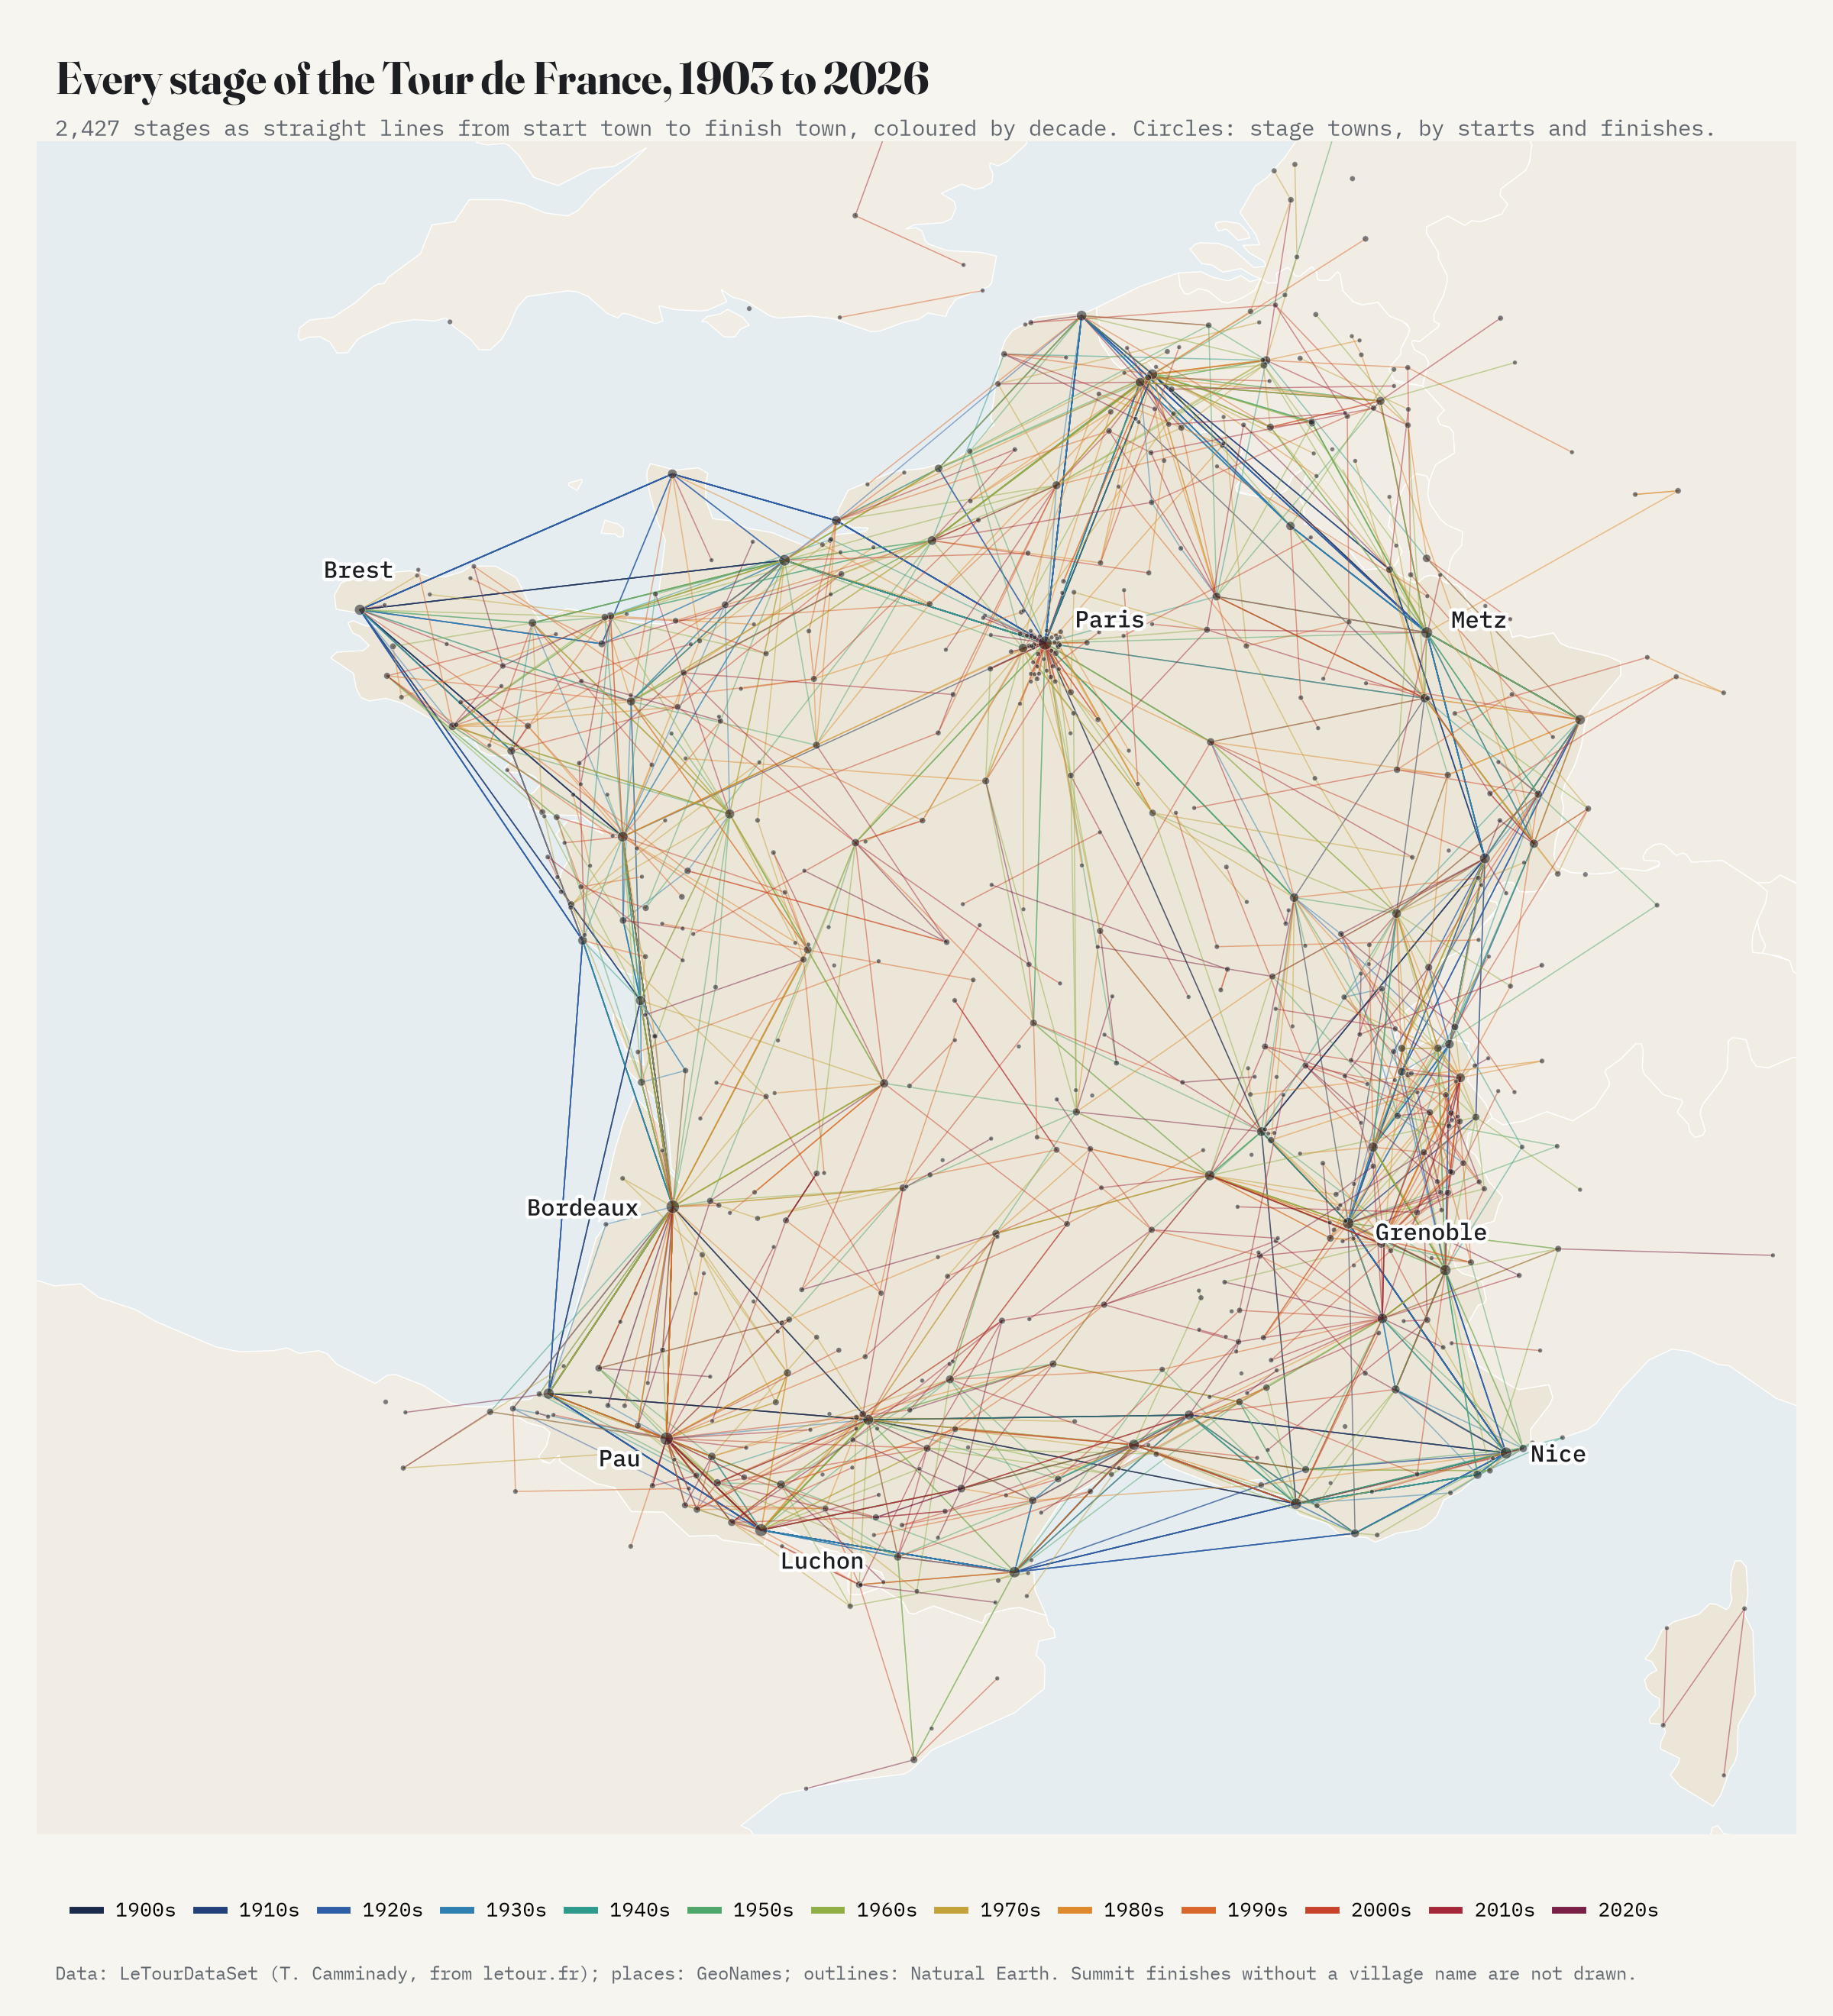
\includegraphics[width=.92\textwidth]{f_map.png}
\caption{Every located stage of the men's Tour, 1903 to 2026, as a straight line from start to finish, coloured by decade. Circles: stage towns, sized by starts and finishes.}\label{fig:map}\end{figure}

\subsection{From a loop to a network}
Figure~\ref{fig:map} shows all located stages. The early decades stand out as thick dark lines round the edge of the country. The 1926 Tour (Figure~\ref{fig:loop}) is the clearest case: 17 stages in a single unbroken loop from Évian, along the eastern frontier to Dunkirk, round Normandy and Brittany, down the Atlantic coast, across the Pyrenees and the Mediterranean, up the Alps and back to Évian and Paris. Measured by stage towns, 92\% of French stage towns in the 1920s lay within 50 km of the edge (median distance 4.2 km), against 37\% of the area. The share fell through the middle of the century and has stayed near half since the 1980s (49\% in the 2020s; median 52.2 km), still above the area share (Figure~\ref{fig:edge}, Table~\ref{tab:decades}).

\begin{figure}[tbp]\centering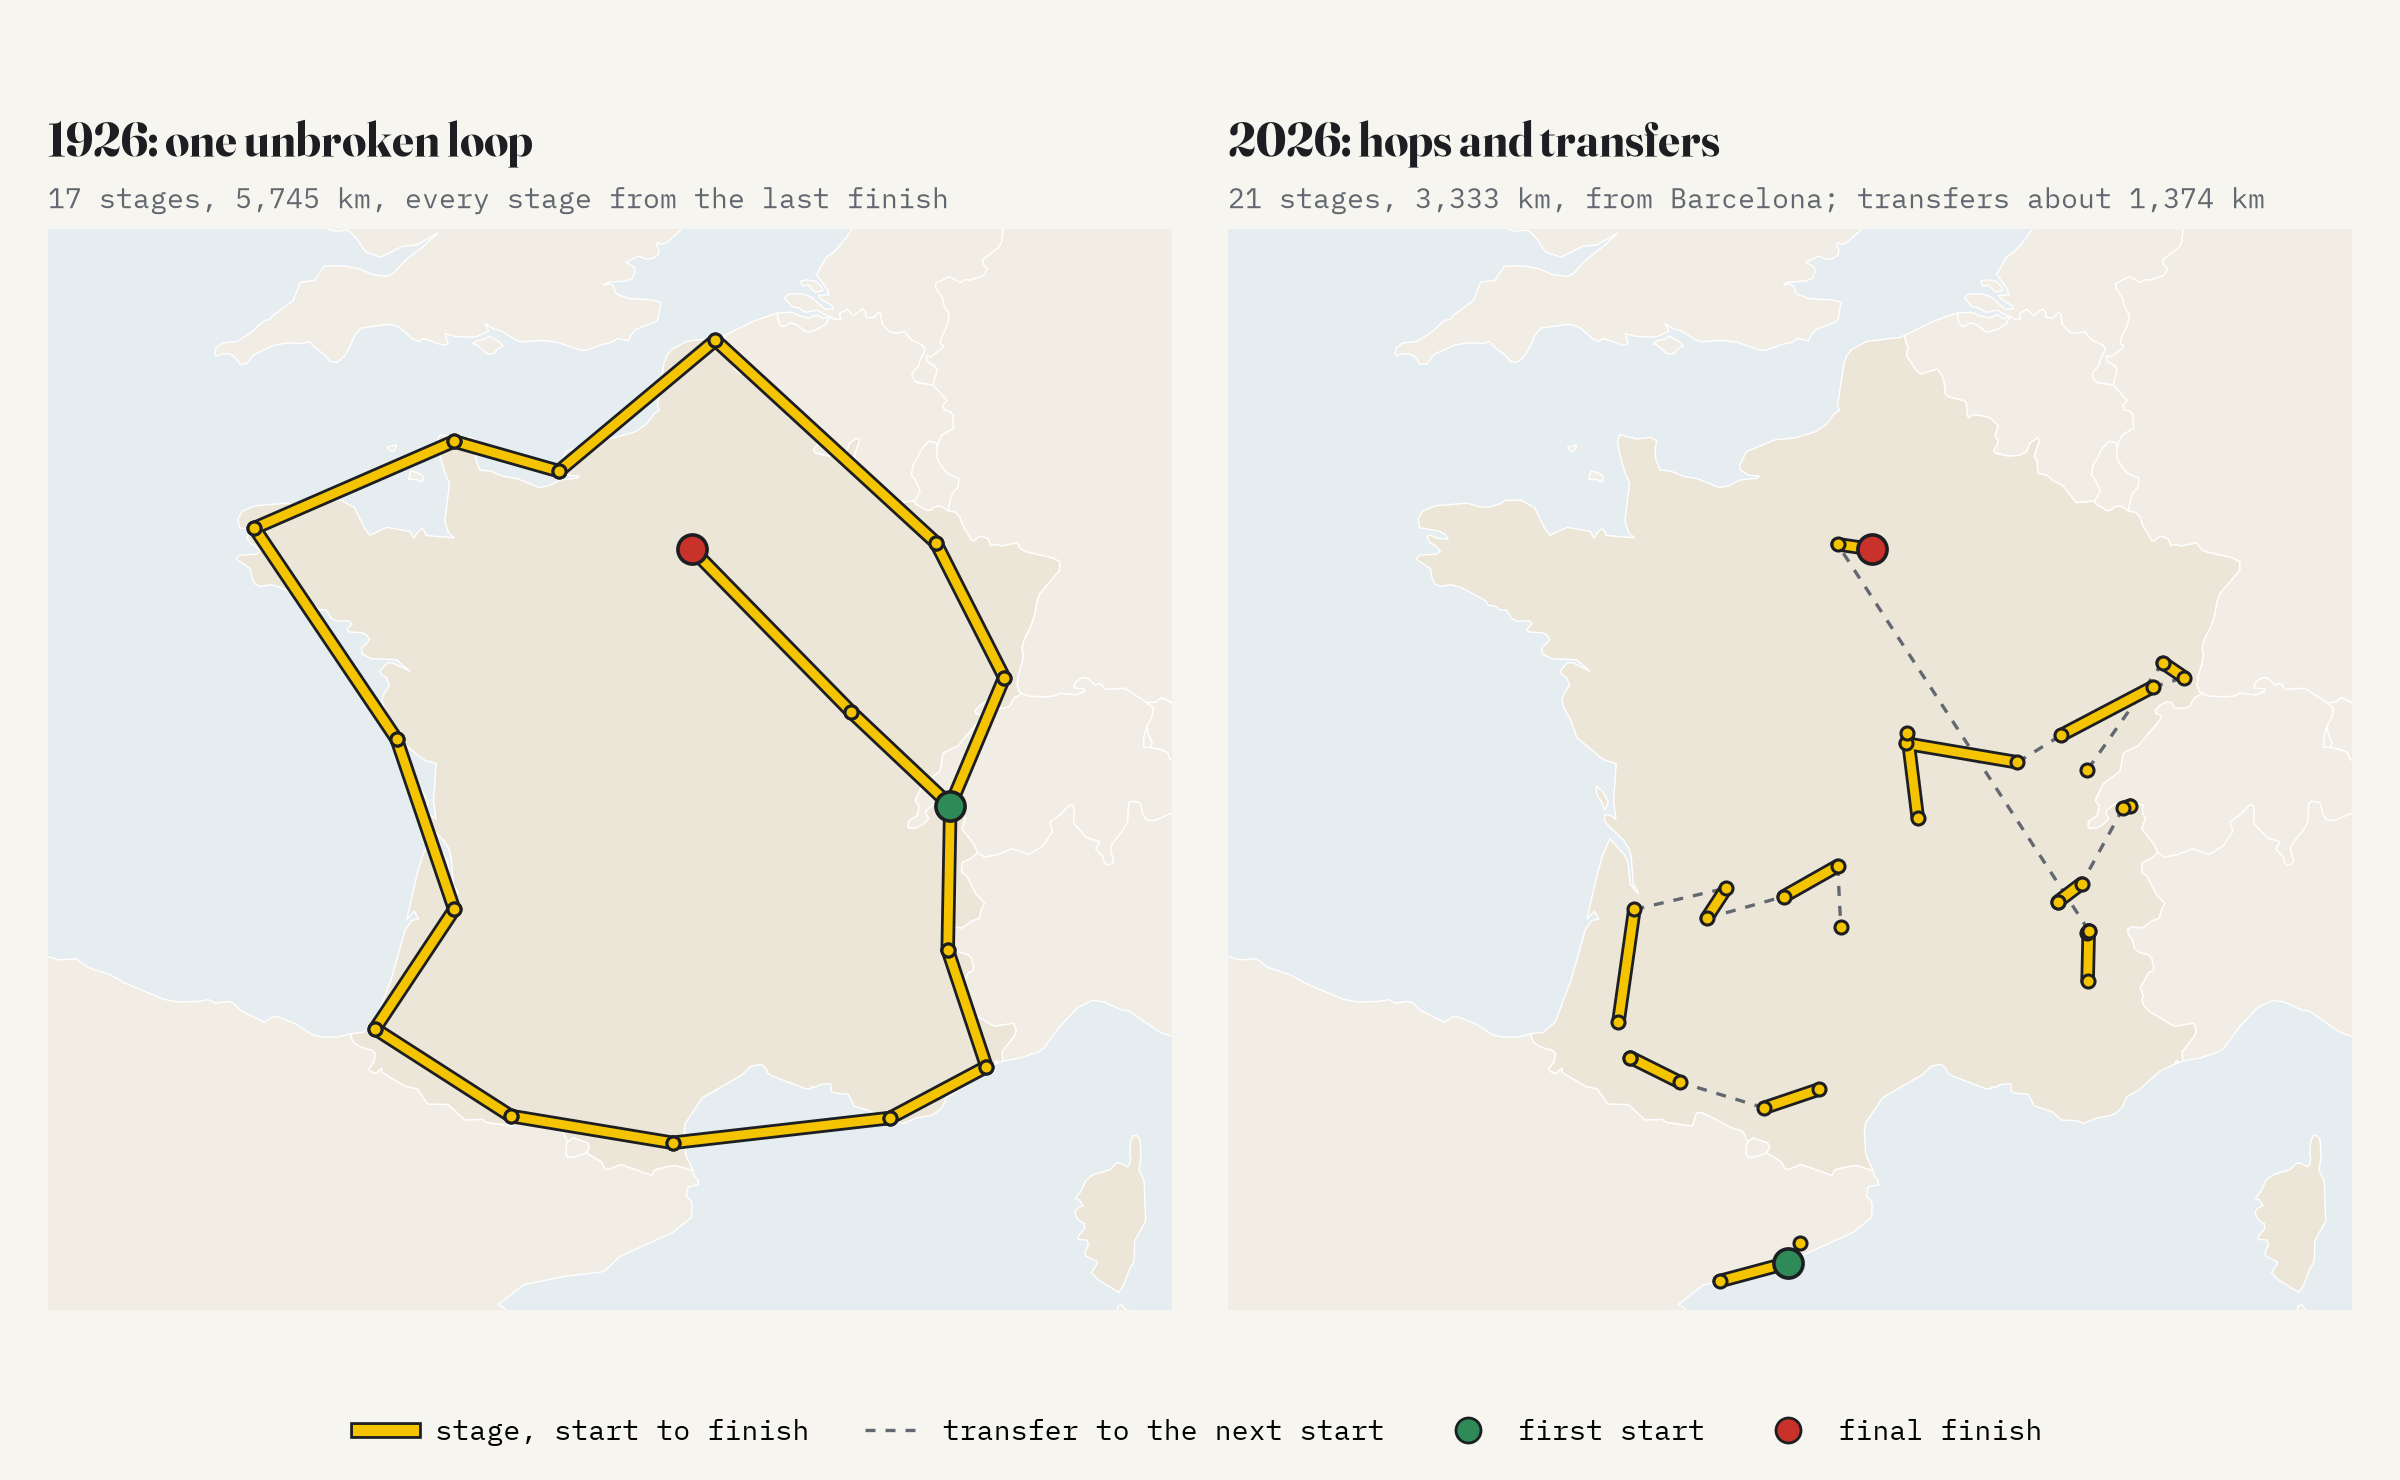
\includegraphics[width=\textwidth]{f_loop.png}
\caption{The 1926 Tour and the 2026 Tour. Yellow: stages; dashed: transfers between a finish and the next start.}\label{fig:loop}\end{figure}

The loop was also continuous. In the 1910s, 1920s and 1930s no stage began anywhere but the previous finish. Transfers stayed rare until the 1950s and then grew steadily: 11.3\% of stages in the 1960s, 40.8\% in the 1980s, 68.4\% in the 2000s and 87.8\% in the 2020s. The last Tour without any transfer between located towns was 1967. Summed as straight lines, transfers averaged 92 km a Tour in the 1950s and 1,152 km in the 2020s, with a maximum of 2,128 km in 2018. The longest single transfer is 681 km, from Espelette to Houilles in 2018.

\begin{figure}[tbp]\centering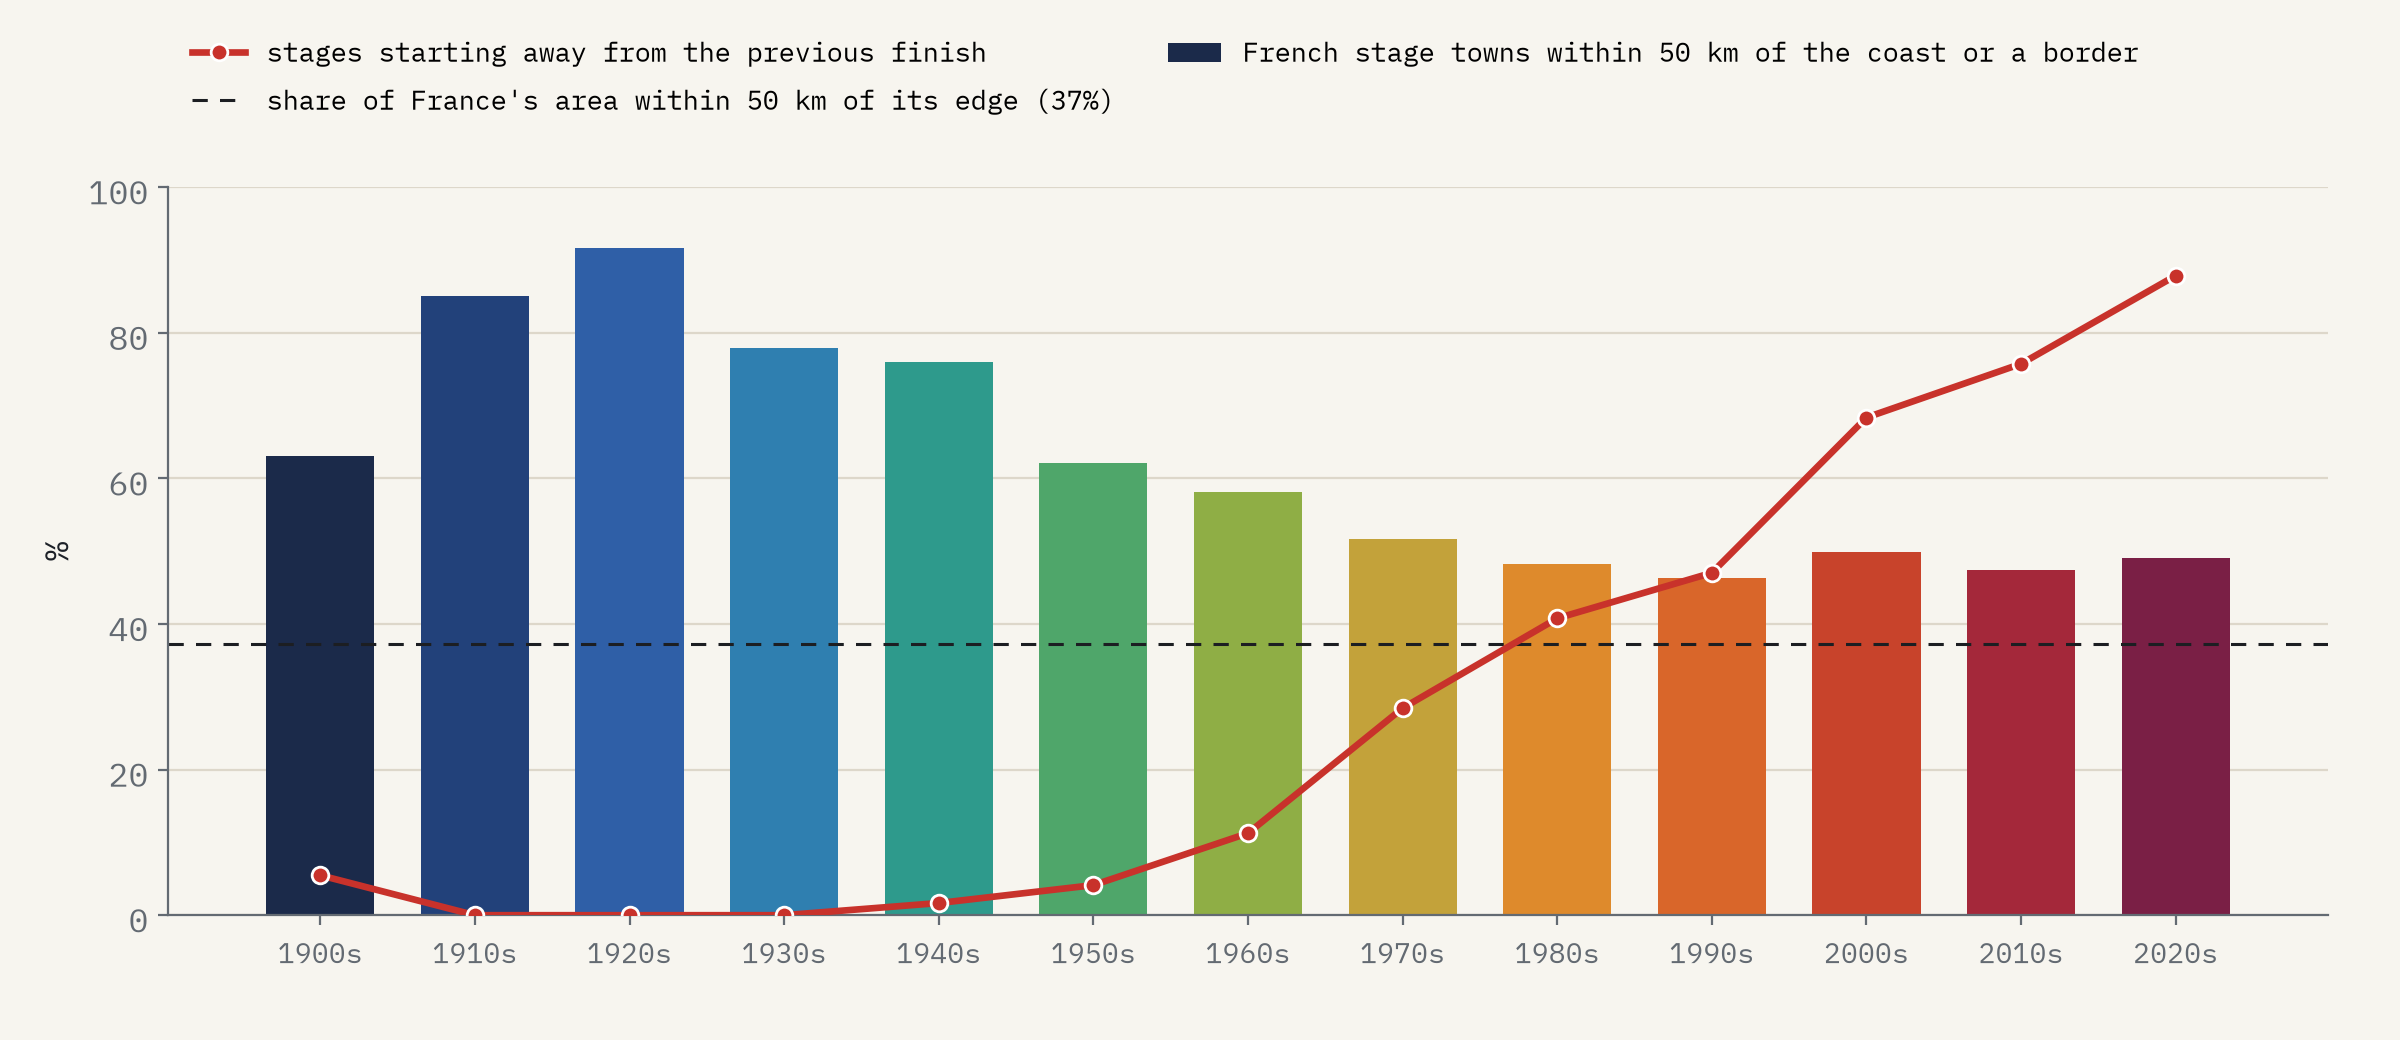
\includegraphics[width=\textwidth]{f_edge.png}
\caption{By decade: share of French stage towns within 50 km of the coast or a land border (bars), share of stages starting away from the previous finish (line), and the share of France's area within 50 km of its edge (dashed).}\label{fig:edge}\end{figure}

\begin{table}[tbp]\centering\small\setlength{\tabcolsep}{5pt}\caption{The men's Tour by decade: Tours, stages, mean total distance (km), mean stage (km), mean winning speed (km/h), stages abroad (\%), stages starting away from the previous finish (\%), and French stage towns within 50 km of the edge of France (\%).}\label{tab:decades}\begin{tabular}{lrrrrrrrr}\toprule Decade & Tours & Stages & km & Stage & km/h & Abroad & Transfer & Edge\\\midrule
1900s & 7 & 80 & 3,709 & 324 & 25.5 & 0.0 & 5.5 & 63.1\\
1910s & 6 & 90 & 5,266 & 351 & 25.9 & 6.7 & 0.0 & 85.1\\
1920s & 10 & 178 & 5,452 & 306 & 25.4 & 3.4 & 0.0 & 91.7\\
1930s & 10 & 255 & 4,537 & 178 & 30.3 & 2.8 & 0.0 & 77.9\\
1940s & 3 & 63 & 4,791 & 228 & 32.3 & 25.4 & 1.7 & 75.9\\
1950s & 10 & 232 & 4,583 & 198 & 34.3 & 17.2 & 4.1 & 62.2\\
1960s & 10 & 242 & 4,339 & 179 & 35.9 & 18.2 & 11.3 & 58.2\\
1970s & 10 & 263 & 3,968 & 151 & 35.4 & 15.2 & 28.4 & 51.7\\
1980s & 10 & 239 & 3,794 & 159 & 37.3 & 11.7 & 40.8 & 48.3\\
1990s & 10 & 218 & 3,819 & 175 & 39.3 & 17.9 & 47.0 & 46.4\\
2000s & 10 & 210 & 3,506 & 167 & 40.2 & 14.3 & 68.4 & 49.9\\
2010s & 10 & 210 & 3,497 & 166 & 40.4 & 13.8 & 75.7 & 47.4\\
2020s & 7 & 147 & 3,392 & 162 & 42.1 & 12.9 & 87.8 & 49.1\\
\bottomrule\end{tabular}\end{table}

\subsection{Distance and speed}
The total distance rose quickly, and every Tour from 1911 to 1929 covered more than 5,000 km; the longest Tour was 1926, at 5,745 km, and the shortest the first two, at 2,428 km (Figure~\ref{fig:distance}). The decade mean fell from 5,452 km in the 1920s to 3,392 km in the 2020s, and the mean stage from 306.3 km to 161.5 km. The six stages of 1903 averaged 405 km; the 31 stages of 1937 were the most in any Tour. The winner's average speed rose from 25.7 km/h in 1903 and 24.1 km/h in 1926 to 34.3 km/h on average in the 1950s and 42.1 km/h in the 2020s; the fastest was 45.08 km/h in 2026. In 1926 the winner rode for 238.7 hours, in 2026 for 73.9. Since the source gives no single stage lengths, the longest stage can be measured only as a straight line: Paris to Lyon in 1903 and 1904, 393 km. The mean straight line across all stages with two located ends is 122.0 km, and 148 stages, mostly time trials and circuits, start and finish in the same place.

\begin{figure}[tbp]\centering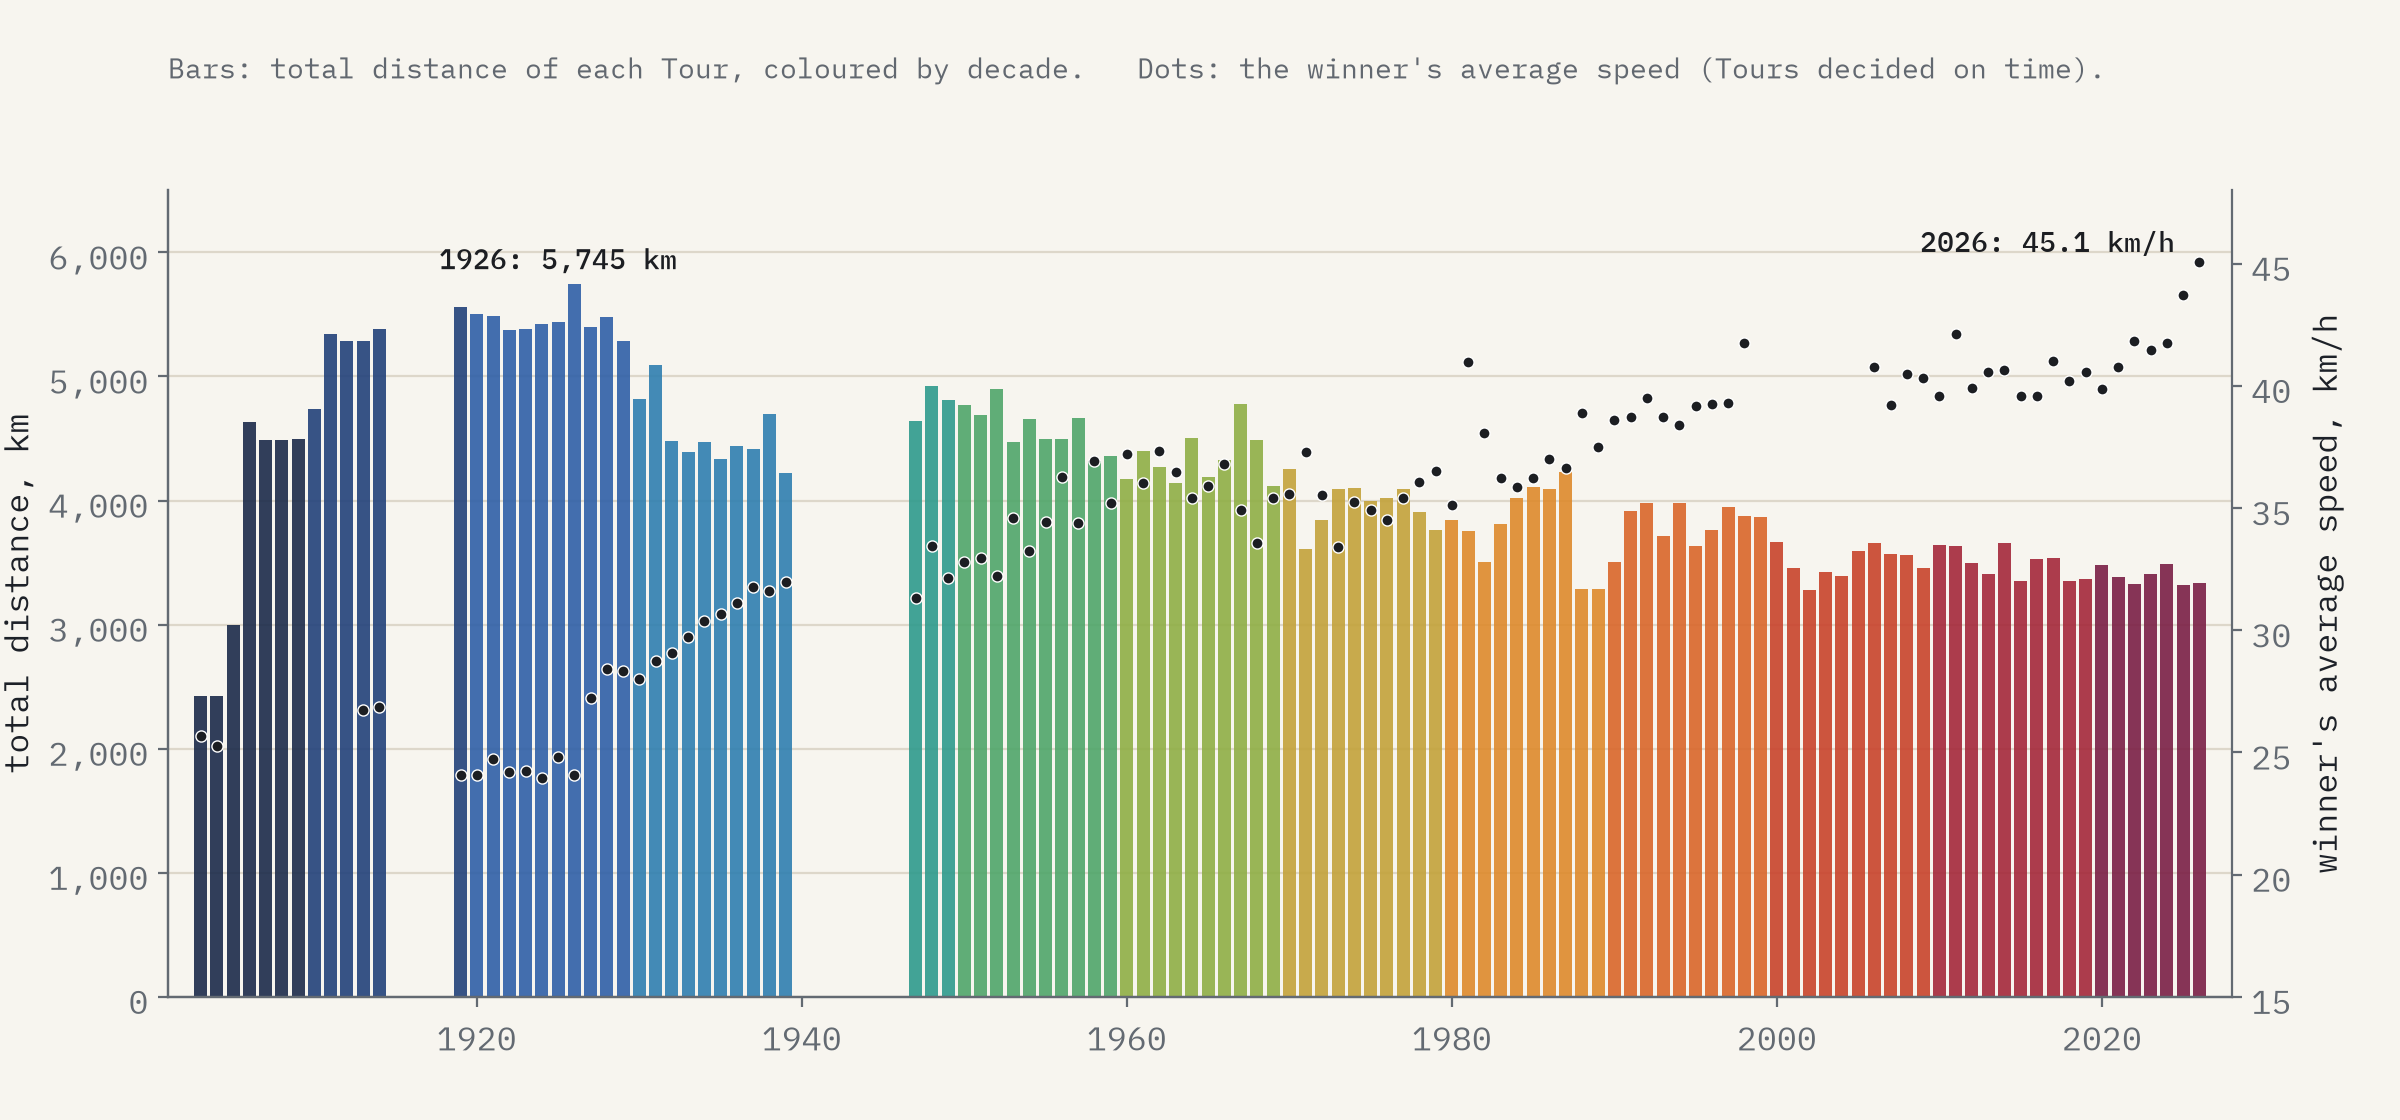
\includegraphics[width=\textwidth]{f_distance.png}
\caption{Total distance of each Tour (bars, coloured by decade) and the overall winner's average speed (dots).}\label{fig:distance}\end{figure}

\subsection{Stage towns}
The men's Tour has used 684 places, 287 of them (42.0\%) only once (Table~\ref{tab:towns}, Figure~\ref{fig:towns}). Paris has 43 starts and 118 finishes in 112 Tours; every Tour has finished there except 2024 (in Nice), and every Tour started there until the first Grand Départ elsewhere, at Évian in 1926. Bordeaux (137), Pau (133, the most common start, 69) and Luchon (113) follow, all gateways to the Pyrenees, which the loop crossed every year in its early decades. The most visited towns abroad are Brussels (25) and Liège (24).

\begin{table}[tbp]\centering\small\caption{The twenty most visited stage towns of the men's Tour.}\label{tab:towns}\begin{tabular}{llrrrrrr}\toprule Town & Country & Starts & Finishes & Total & Tours & First & Last\\\midrule
Paris & France & 43 & 118 & 161 & 112 & 1903 & 2026\\
Bordeaux & France & 56 & 81 & 137 & 77 & 1903 & 2026\\
Pau & France & 69 & 64 & 133 & 77 & 1930 & 2026\\
Luchon & France & 56 & 57 & 113 & 57 & 1910 & 2025\\
Nice & France & 41 & 37 & 78 & 36 & 1906 & 2024\\
Metz & France & 39 & 38 & 77 & 41 & 1907 & 2012\\
Grenoble & France & 41 & 35 & 76 & 41 & 1905 & 2020\\
Caen & France & 36 & 35 & 71 & 35 & 1905 & 2025\\
Perpignan & France & 34 & 34 & 68 & 36 & 1910 & 2009\\
Marseille & France & 33 & 35 & 68 & 36 & 1903 & 2017\\
Briançon & France & 34 & 32 & 66 & 35 & 1922 & 2022\\
Bayonne & France & 31 & 31 & 62 & 33 & 1906 & 2023\\
Montpellier & France & 30 & 30 & 60 & 33 & 1930 & 2025\\
Brest & France & 30 & 27 & 57 & 31 & 1906 & 2021\\
Belfort & France & 31 & 23 & 54 & 33 & 1907 & 2026\\
Nantes & France & 25 & 29 & 54 & 31 & 1903 & 2008\\
Toulouse & France & 27 & 27 & 54 & 28 & 1903 & 2025\\
Gap & France & 26 & 24 & 50 & 27 & 1931 & 2026\\
Roubaix & France & 26 & 24 & 50 & 26 & 1907 & 2018\\
Dunkirk & France & 25 & 24 & 49 & 26 & 1911 & 2025\\
\bottomrule\end{tabular}\end{table}

\begin{figure}[tbp]\centering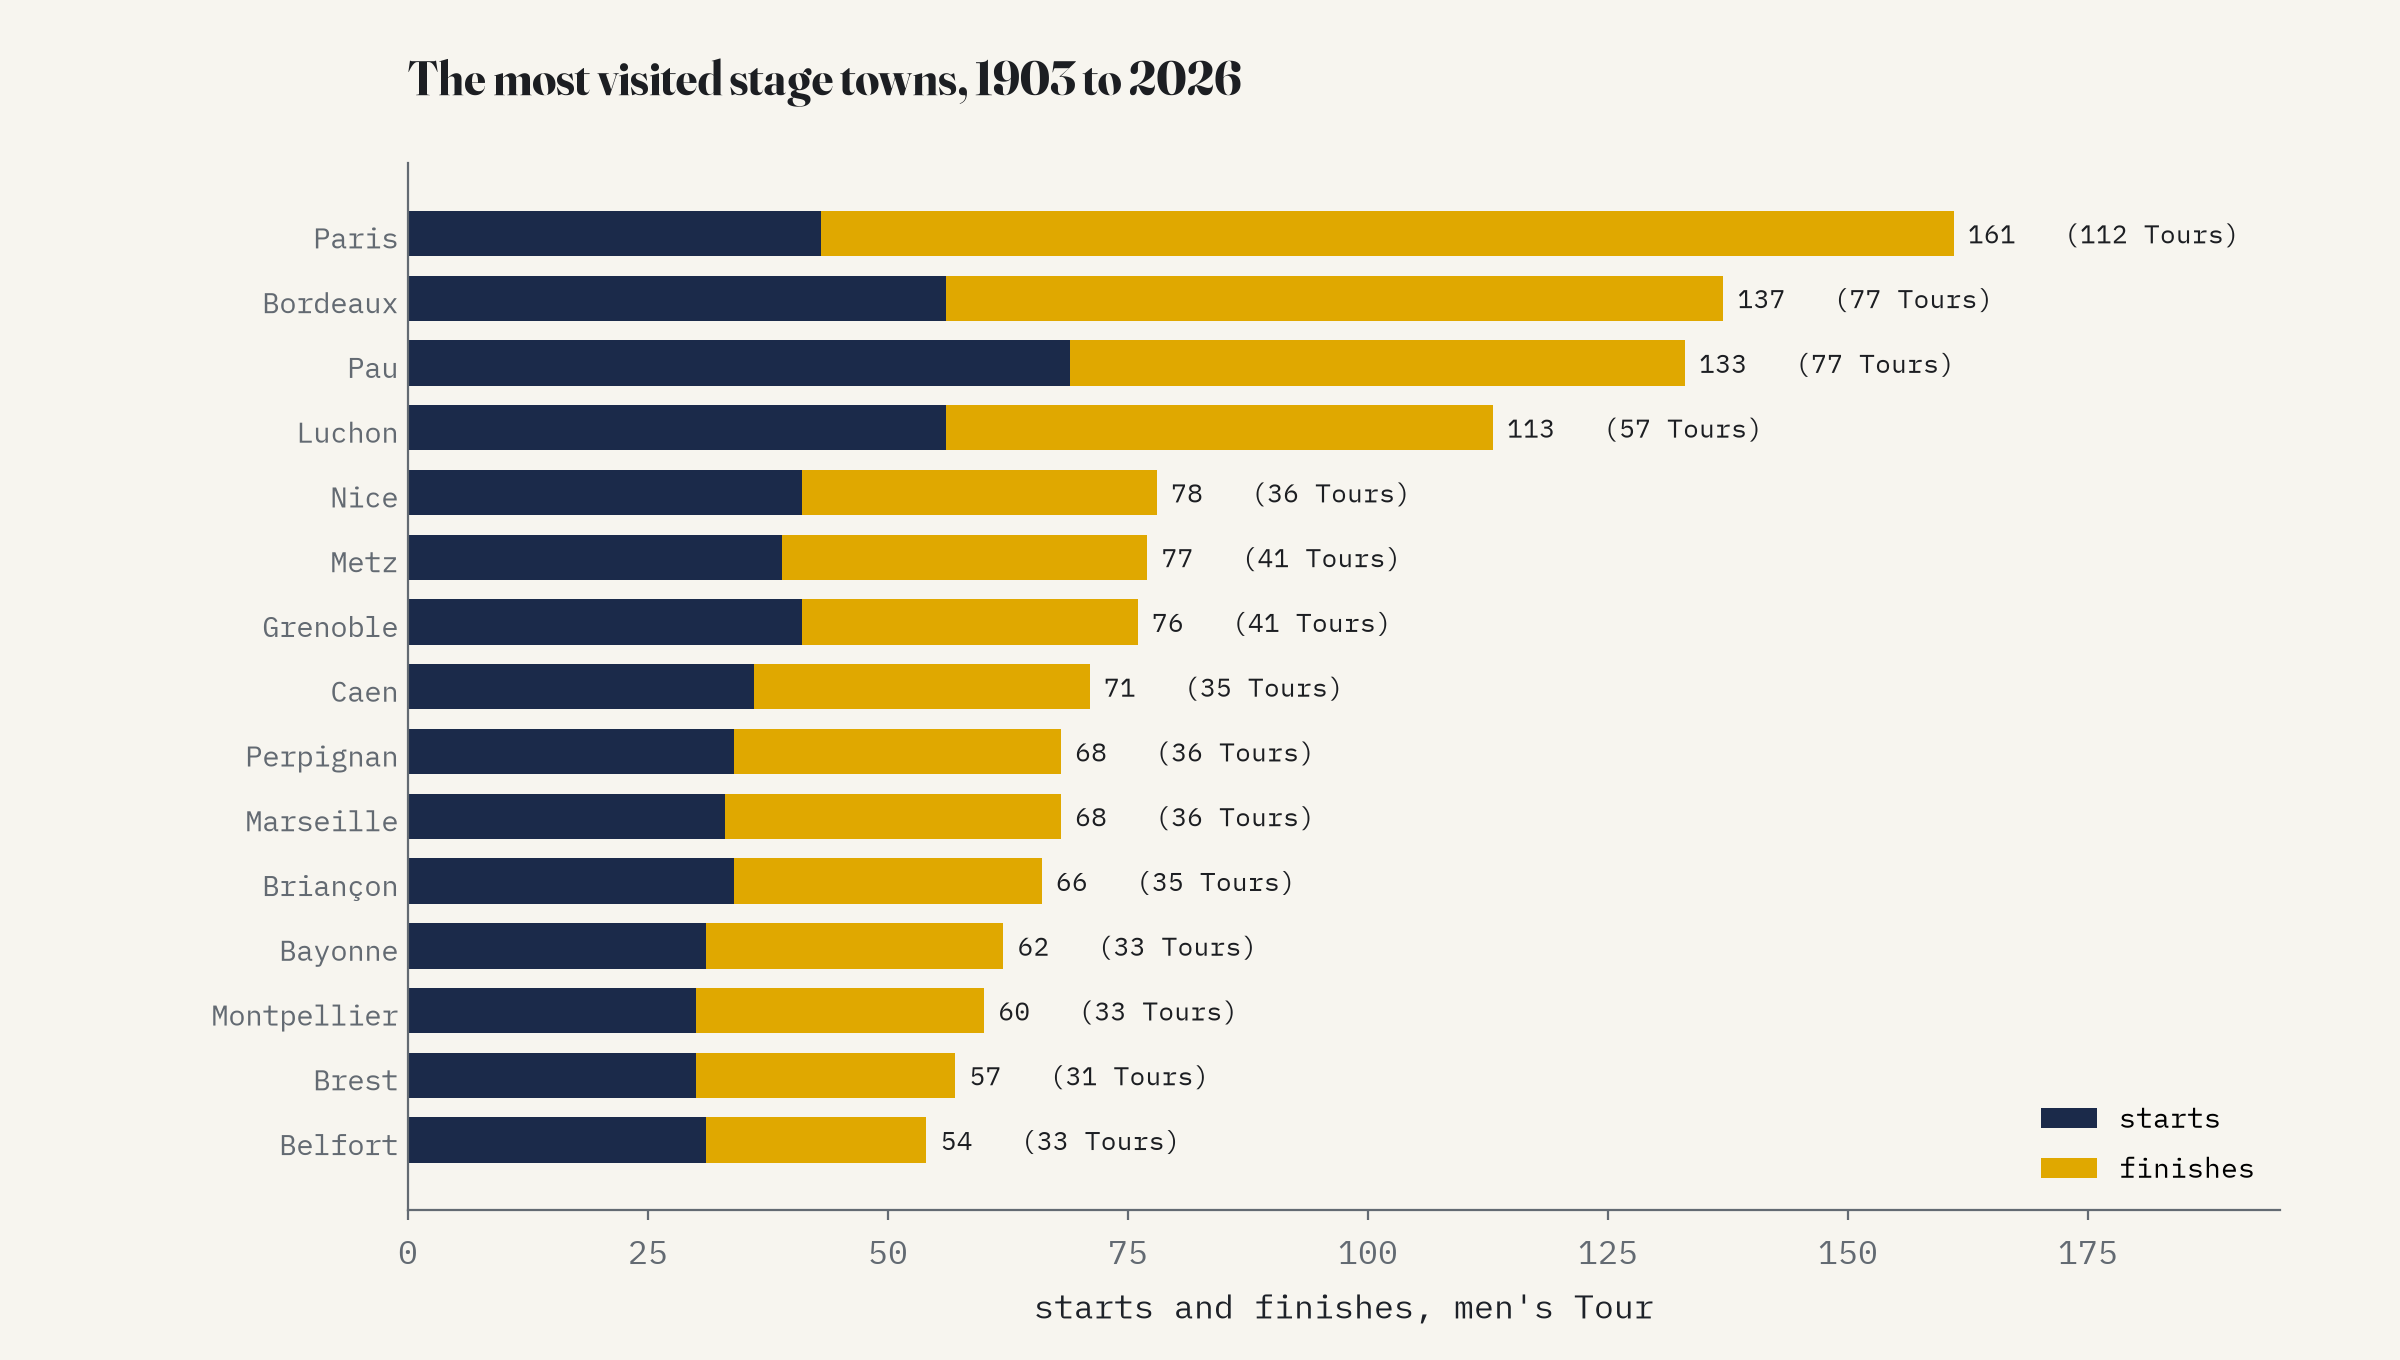
\includegraphics[width=\textwidth]{f_towns.png}
\caption{The fifteen most visited stage towns: starts and finishes, and the number of Tours.}\label{fig:towns}\end{figure}

\subsection{Départements}
Every one of the 96 départements of metropolitan France hosted at least one located start or finish (Figure~\ref{fig:deps}). The busiest is Pyrénées-Atlantiques (228 starts and finishes in 102 Tours), followed by Haute-Garonne (224). The least visited are Deux-Sèvres, where only Niort in 1950 appears among the located towns, and the two Corsican départements, visited once, by the 100th Tour in 2013. Because the data record only starts and finishes, a département that a stage crossed without stopping is not counted.

\begin{figure}[tbp]\centering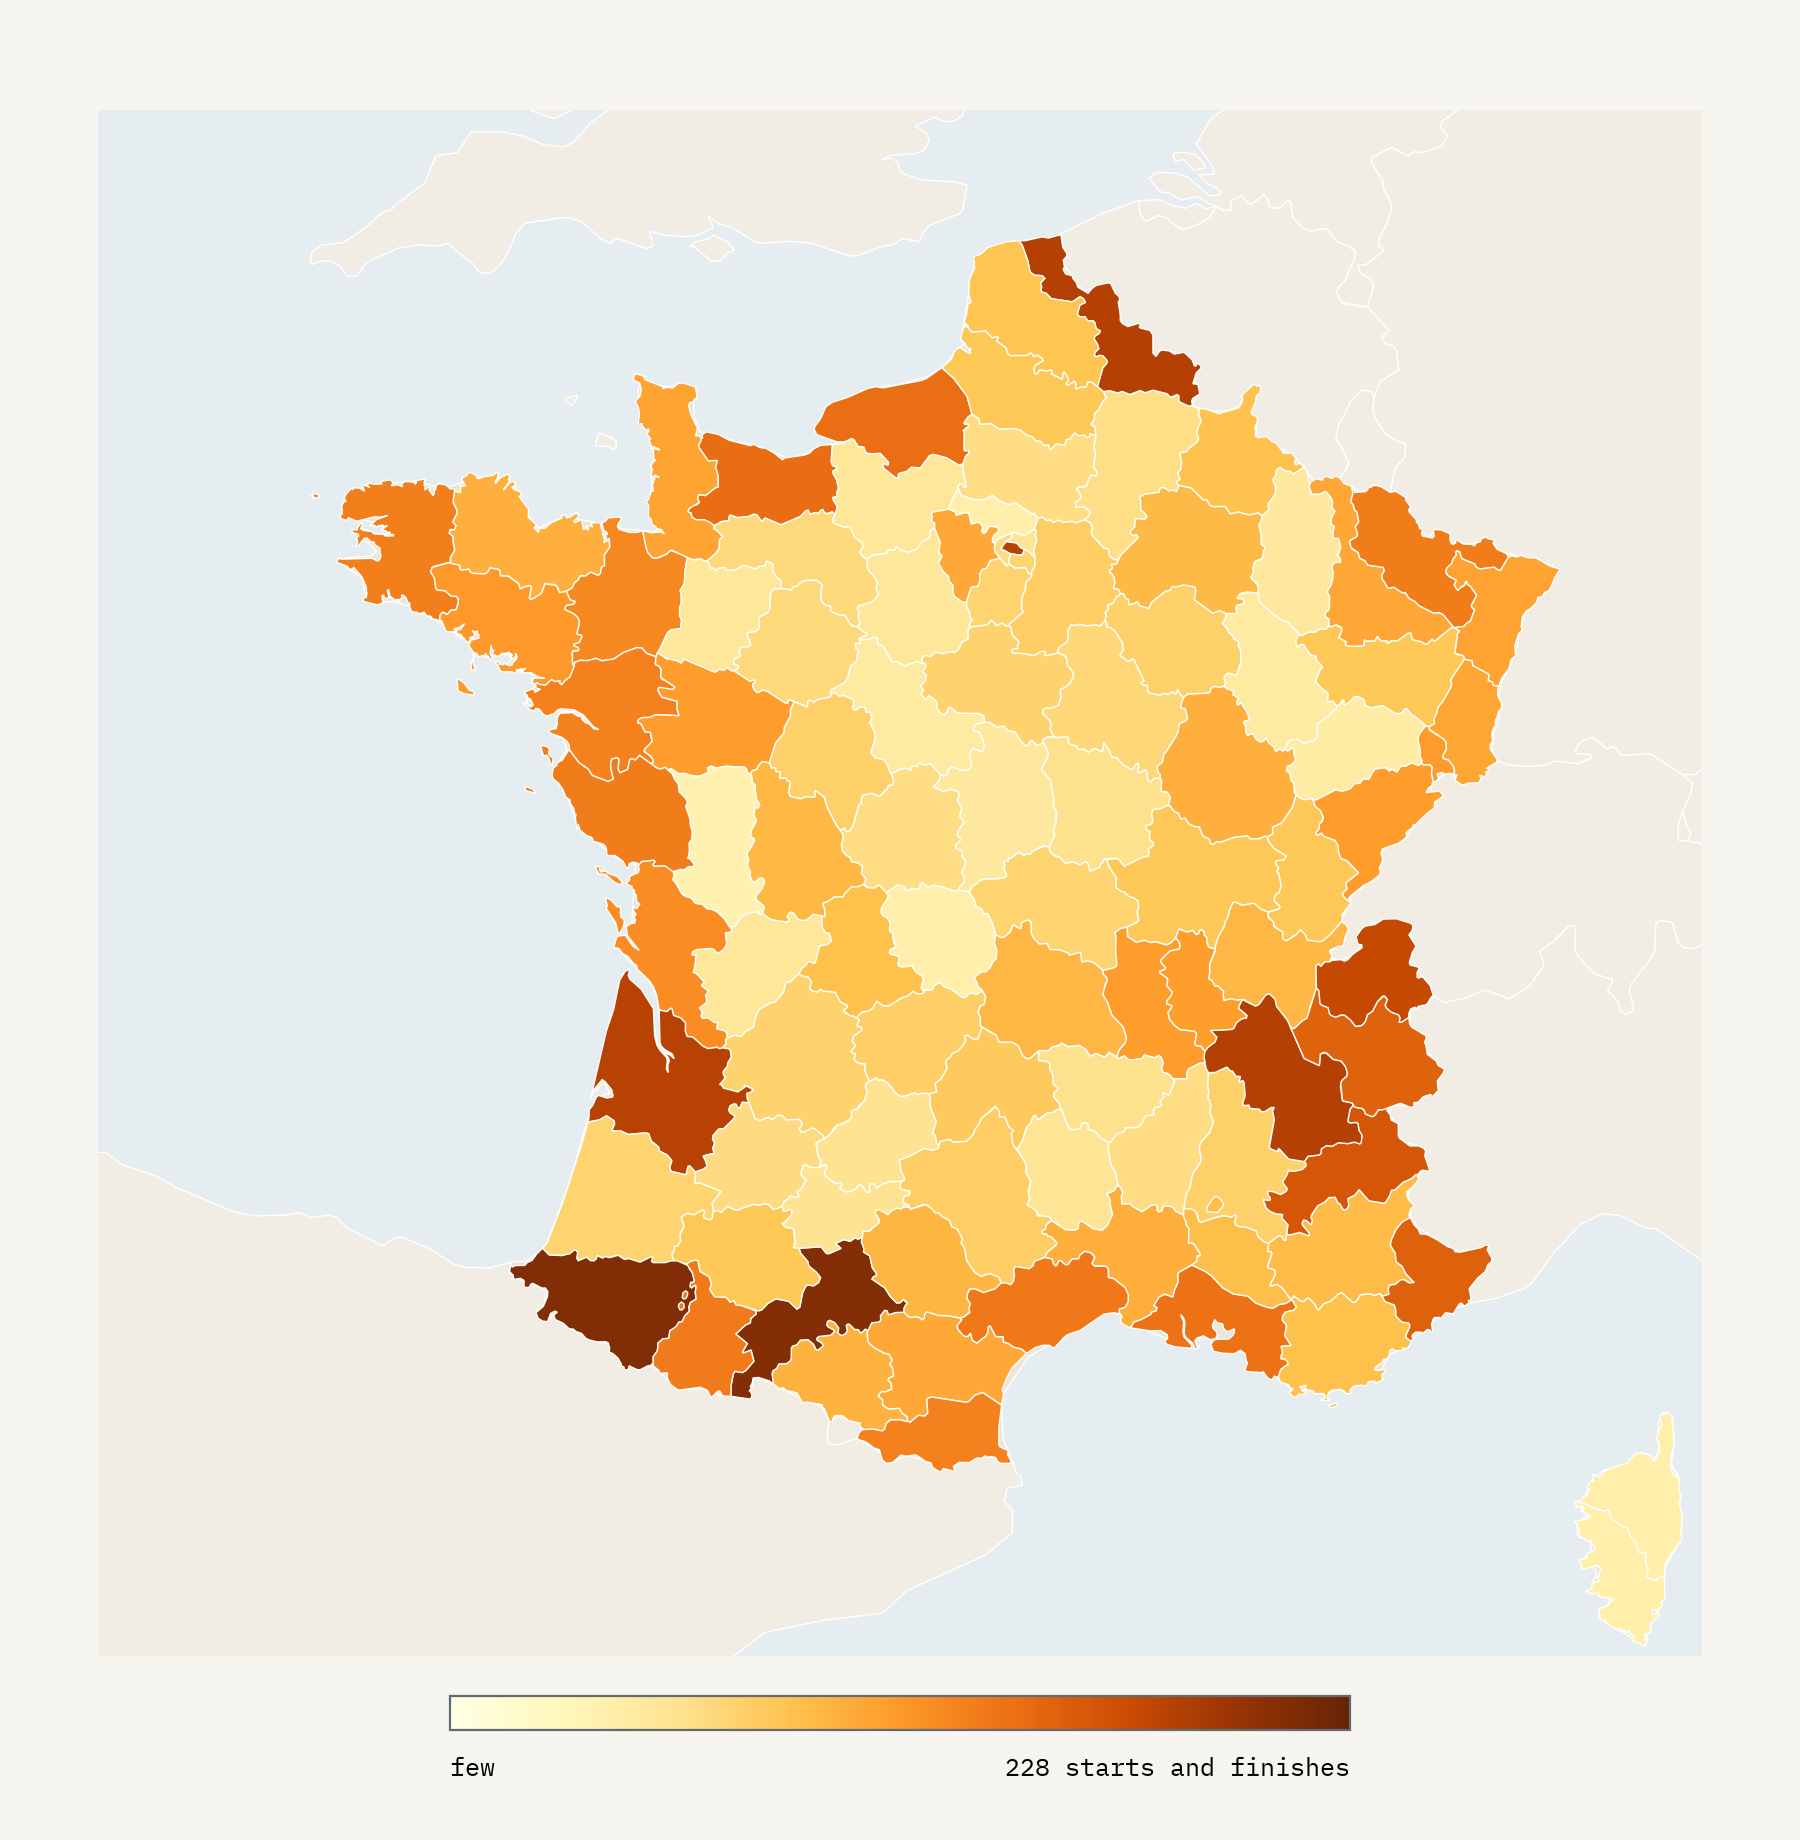
\includegraphics[width=.75\textwidth]{f_deps.png}
\caption{Starts and finishes per département of metropolitan France, men's and women's Tours.}\label{fig:deps}\end{figure}

\subsection{Abroad}
The first stage abroad ran from Grenoble to Geneva in 1913. 304 stages (12.5\%) started or finished in one of 12 other countries, 107 of them with both ends abroad, and 209 (9.3\% of stages with both ends located) crossed a border. Belgium (118 stages), Switzerland (51), Spain (29) and Italy (27) lead (Figure~\ref{fig:abroad}). 34 Tours never left France at their located starts and finishes. The 27 Grand Départs abroad (Table~\ref{tab:gd}) began in Amsterdam in 1954; the Netherlands has had 6, Belgium 5 and Germany 4. Since 2000, 14 of 27 Tours (52\%) started abroad.

\begin{figure}[tbp]\centering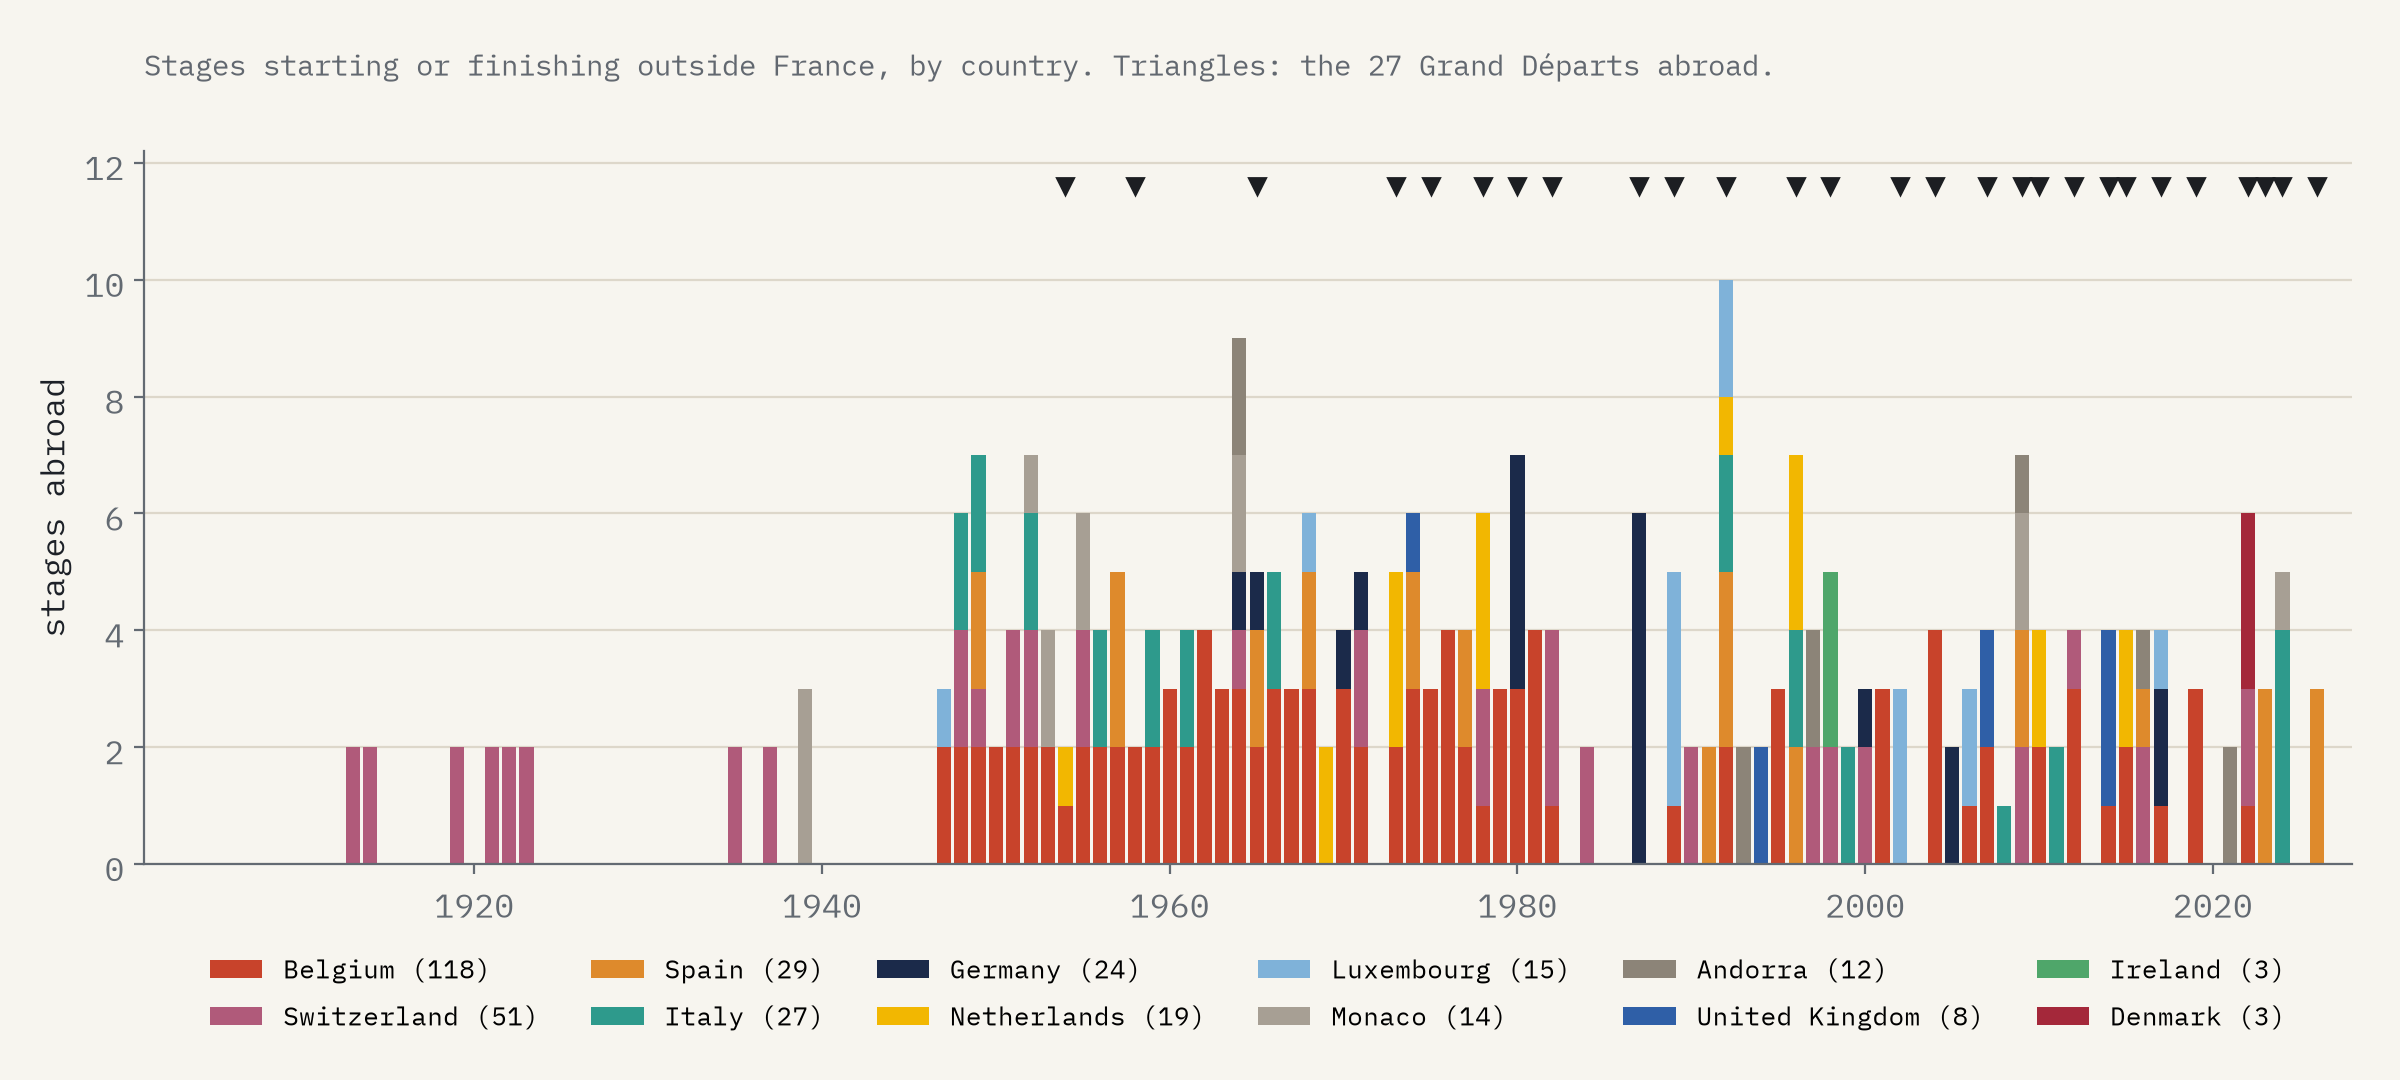
\includegraphics[width=\textwidth]{f_abroad.png}
\caption{Stages starting or finishing outside France, by country, per Tour. Triangles mark Grand Départs abroad.}\label{fig:abroad}\end{figure}

\begin{table}[tbp]\centering\small\caption{Grand Départs outside France: the start town of the first stage or prologue.}\label{tab:gd}\begin{tabular}{rllrll}\toprule Year & Town & Country & Year & Town & Country\\\midrule
1954 & Amsterdam & Netherlands & 2004 & Liège & Belgium\\
1958 & Brussels & Belgium & 2007 & London & United Kingdom\\
1965 & Cologne & Germany & 2009 & Monaco & Monaco\\
1973 & Scheveningen & Netherlands & 2010 & Rotterdam & Netherlands\\
1975 & Charleroi & Belgium & 2012 & Liège & Belgium\\
1978 & Leiden & Netherlands & 2014 & Leeds & United Kingdom\\
1980 & Frankfurt am Main & Germany & 2015 & Utrecht & Netherlands\\
1982 & Basel & Switzerland & 2017 & Düsseldorf & Germany\\
1987 & Berlin & Germany & 2019 & Brussels & Belgium\\
1989 & Luxembourg & Luxembourg & 2022 & Copenhagen & Denmark\\
1992 & San Sebastián & Spain & 2023 & Bilbao & Spain\\
1996 & 's-Hertogenbosch & Netherlands & 2024 & Florence & Italy\\
1998 & Dublin & Ireland & 2026 & Barcelona & Spain\\
2002 & Luxembourg & Luxembourg &  & & \\
\bottomrule\end{tabular}\end{table}

\subsection{Winners}
Of the 106 men's editions with a winner in the official record, French riders won 36, the last in 1985; Belgians 18, the last in 1976; Spaniards 12; Italians 10; British riders 6; and riders from Luxembourg and Slovenia 5 each (Figure~\ref{fig:winners}). The first winner from outside France came in 1909 and the first from outside Europe in 1986. Jacques Anquetil, Eddy Merckx, Bernard Hinault, Miguel Indurain and Tadej Pogačar won five times each. The record has no winner for 1999 to 2005: Lance Armstrong's seven titles were stripped in 2012 and not reawarded. For 2006 and 2010 it lists Óscar Pereiro and Andy Schleck, who received the titles after the original winners were disqualified. I report the record as the source gives it.

\begin{figure}[tbp]\centering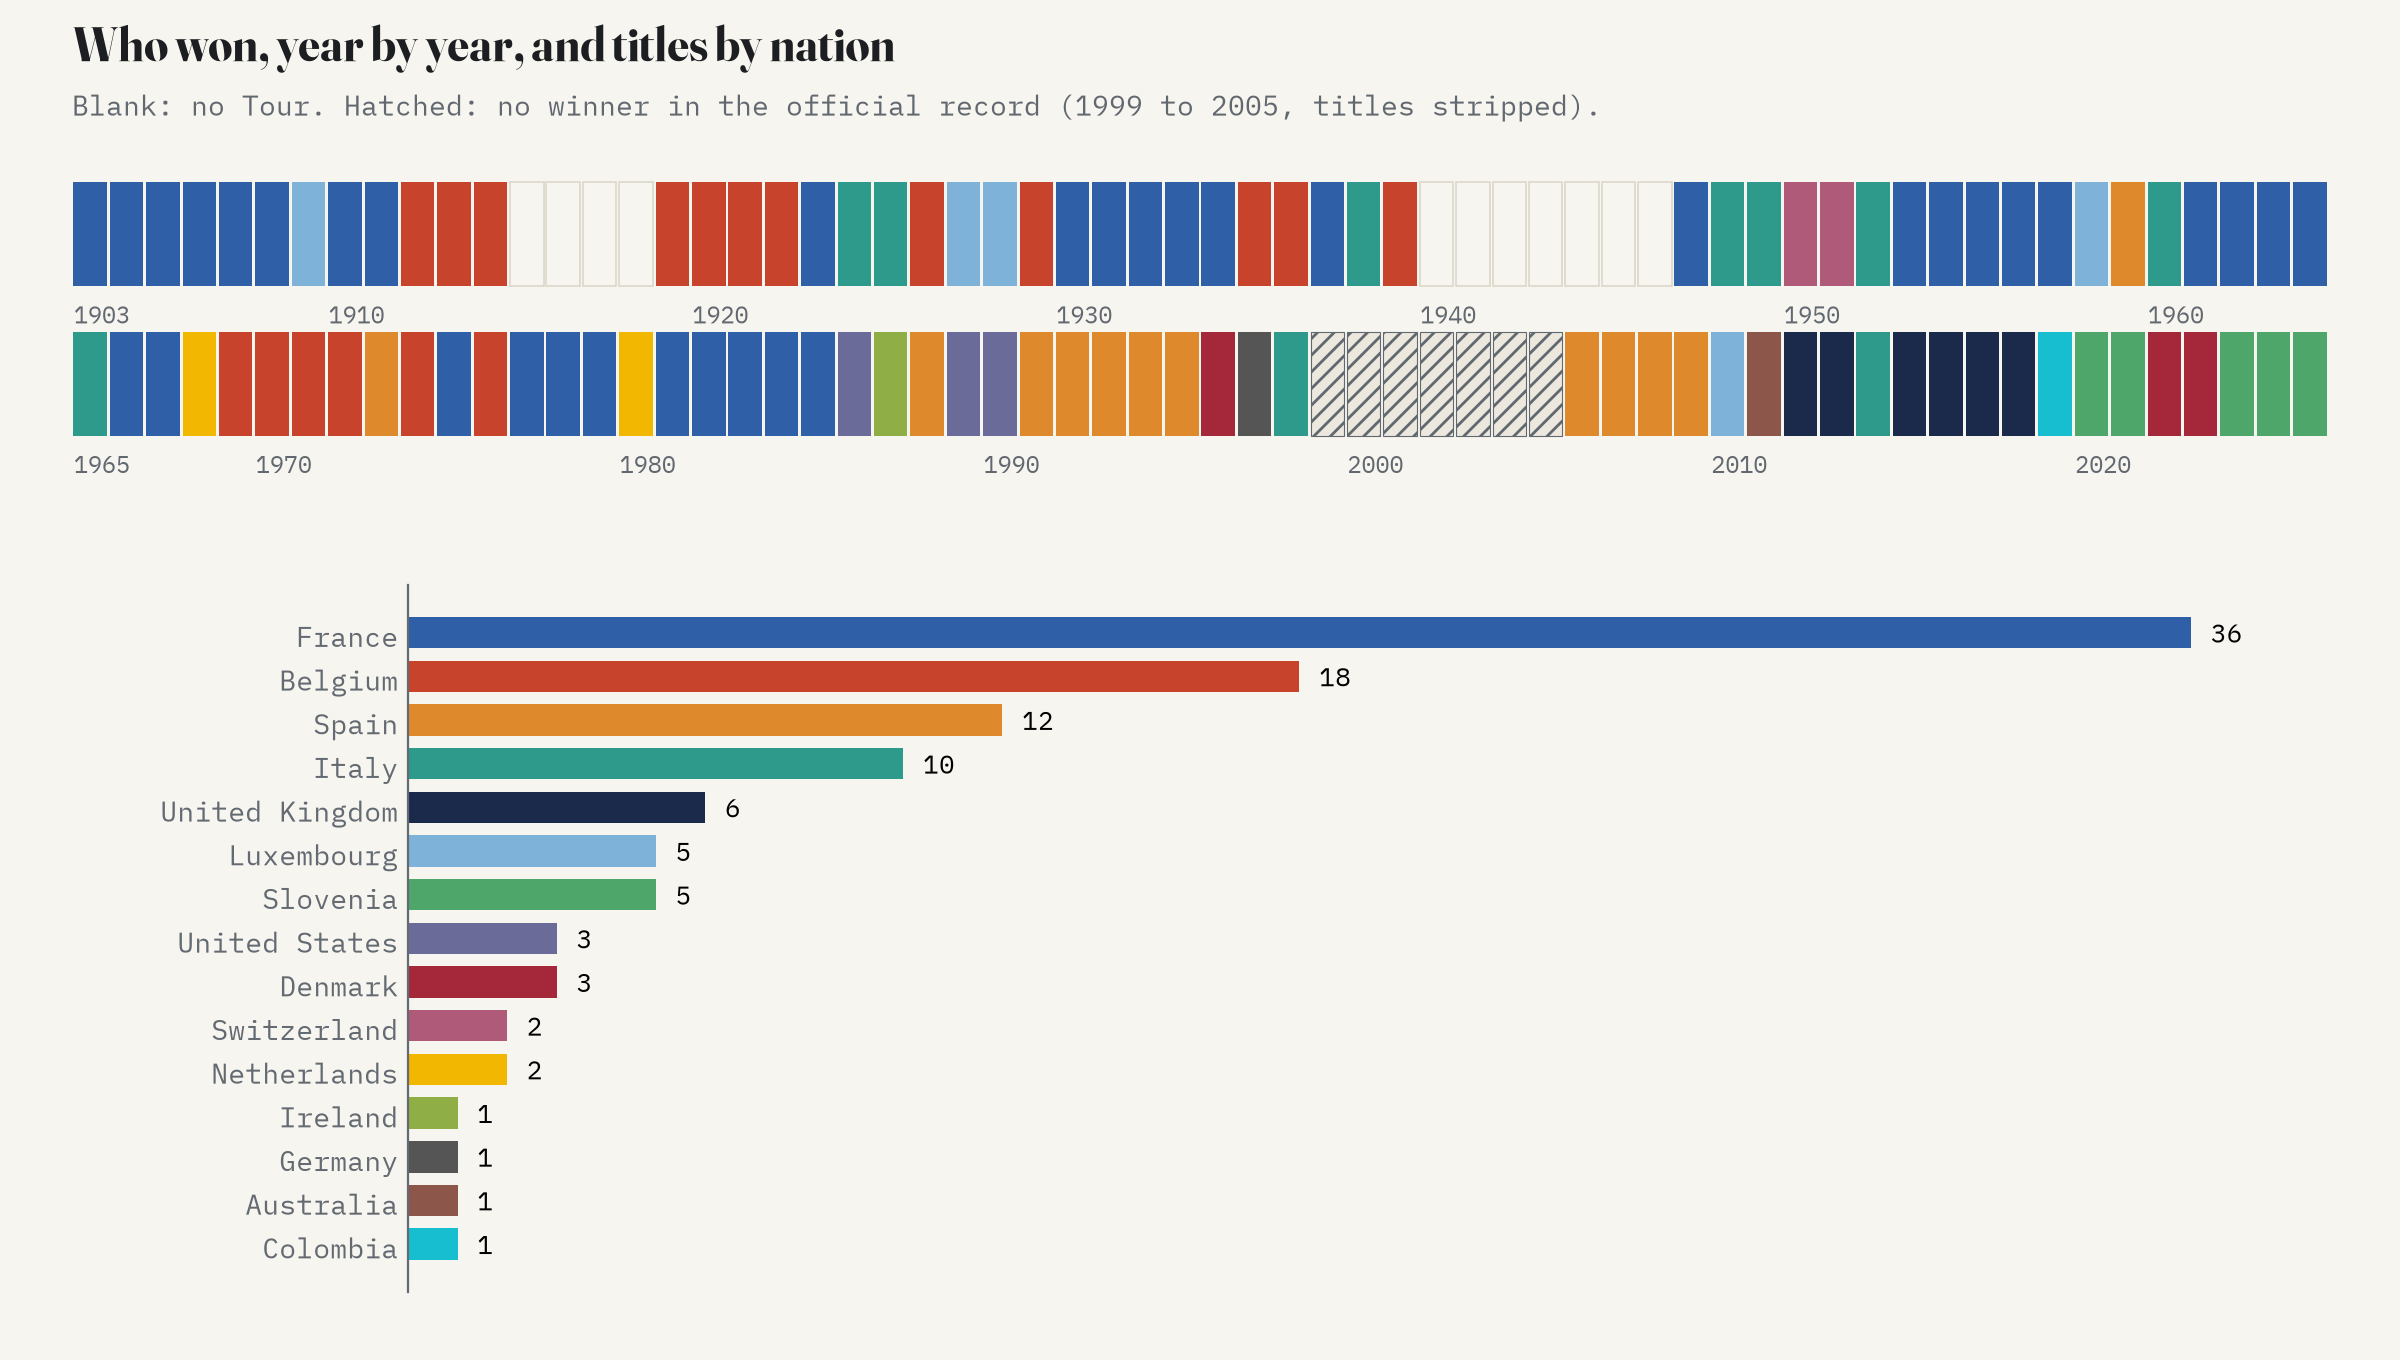
\includegraphics[width=\textwidth]{f_winners.png}
\caption{The winner's nation, year by year (blank: no Tour; hatched: no winner in the official record), and titles by nation.}\label{fig:winners}\end{figure}

\subsection{The Tour de France Femmes}
The women's race, relaunched in 2022, has run 5 times with 42 stages and 5,275 km in all (Figure~\ref{fig:women}). It has used 63 places in 37 départements, 46 of them shared with the men's race, and started abroad twice, in Rotterdam (2024) and Lausanne (2026). The winners were Annemiek van Vleuten (2022), Demi Vollering (2023, 2026), Katarzyna Niewiadoma (2024) and Pauline Ferrand-Prévot (2025).

\begin{figure}[tbp]\centering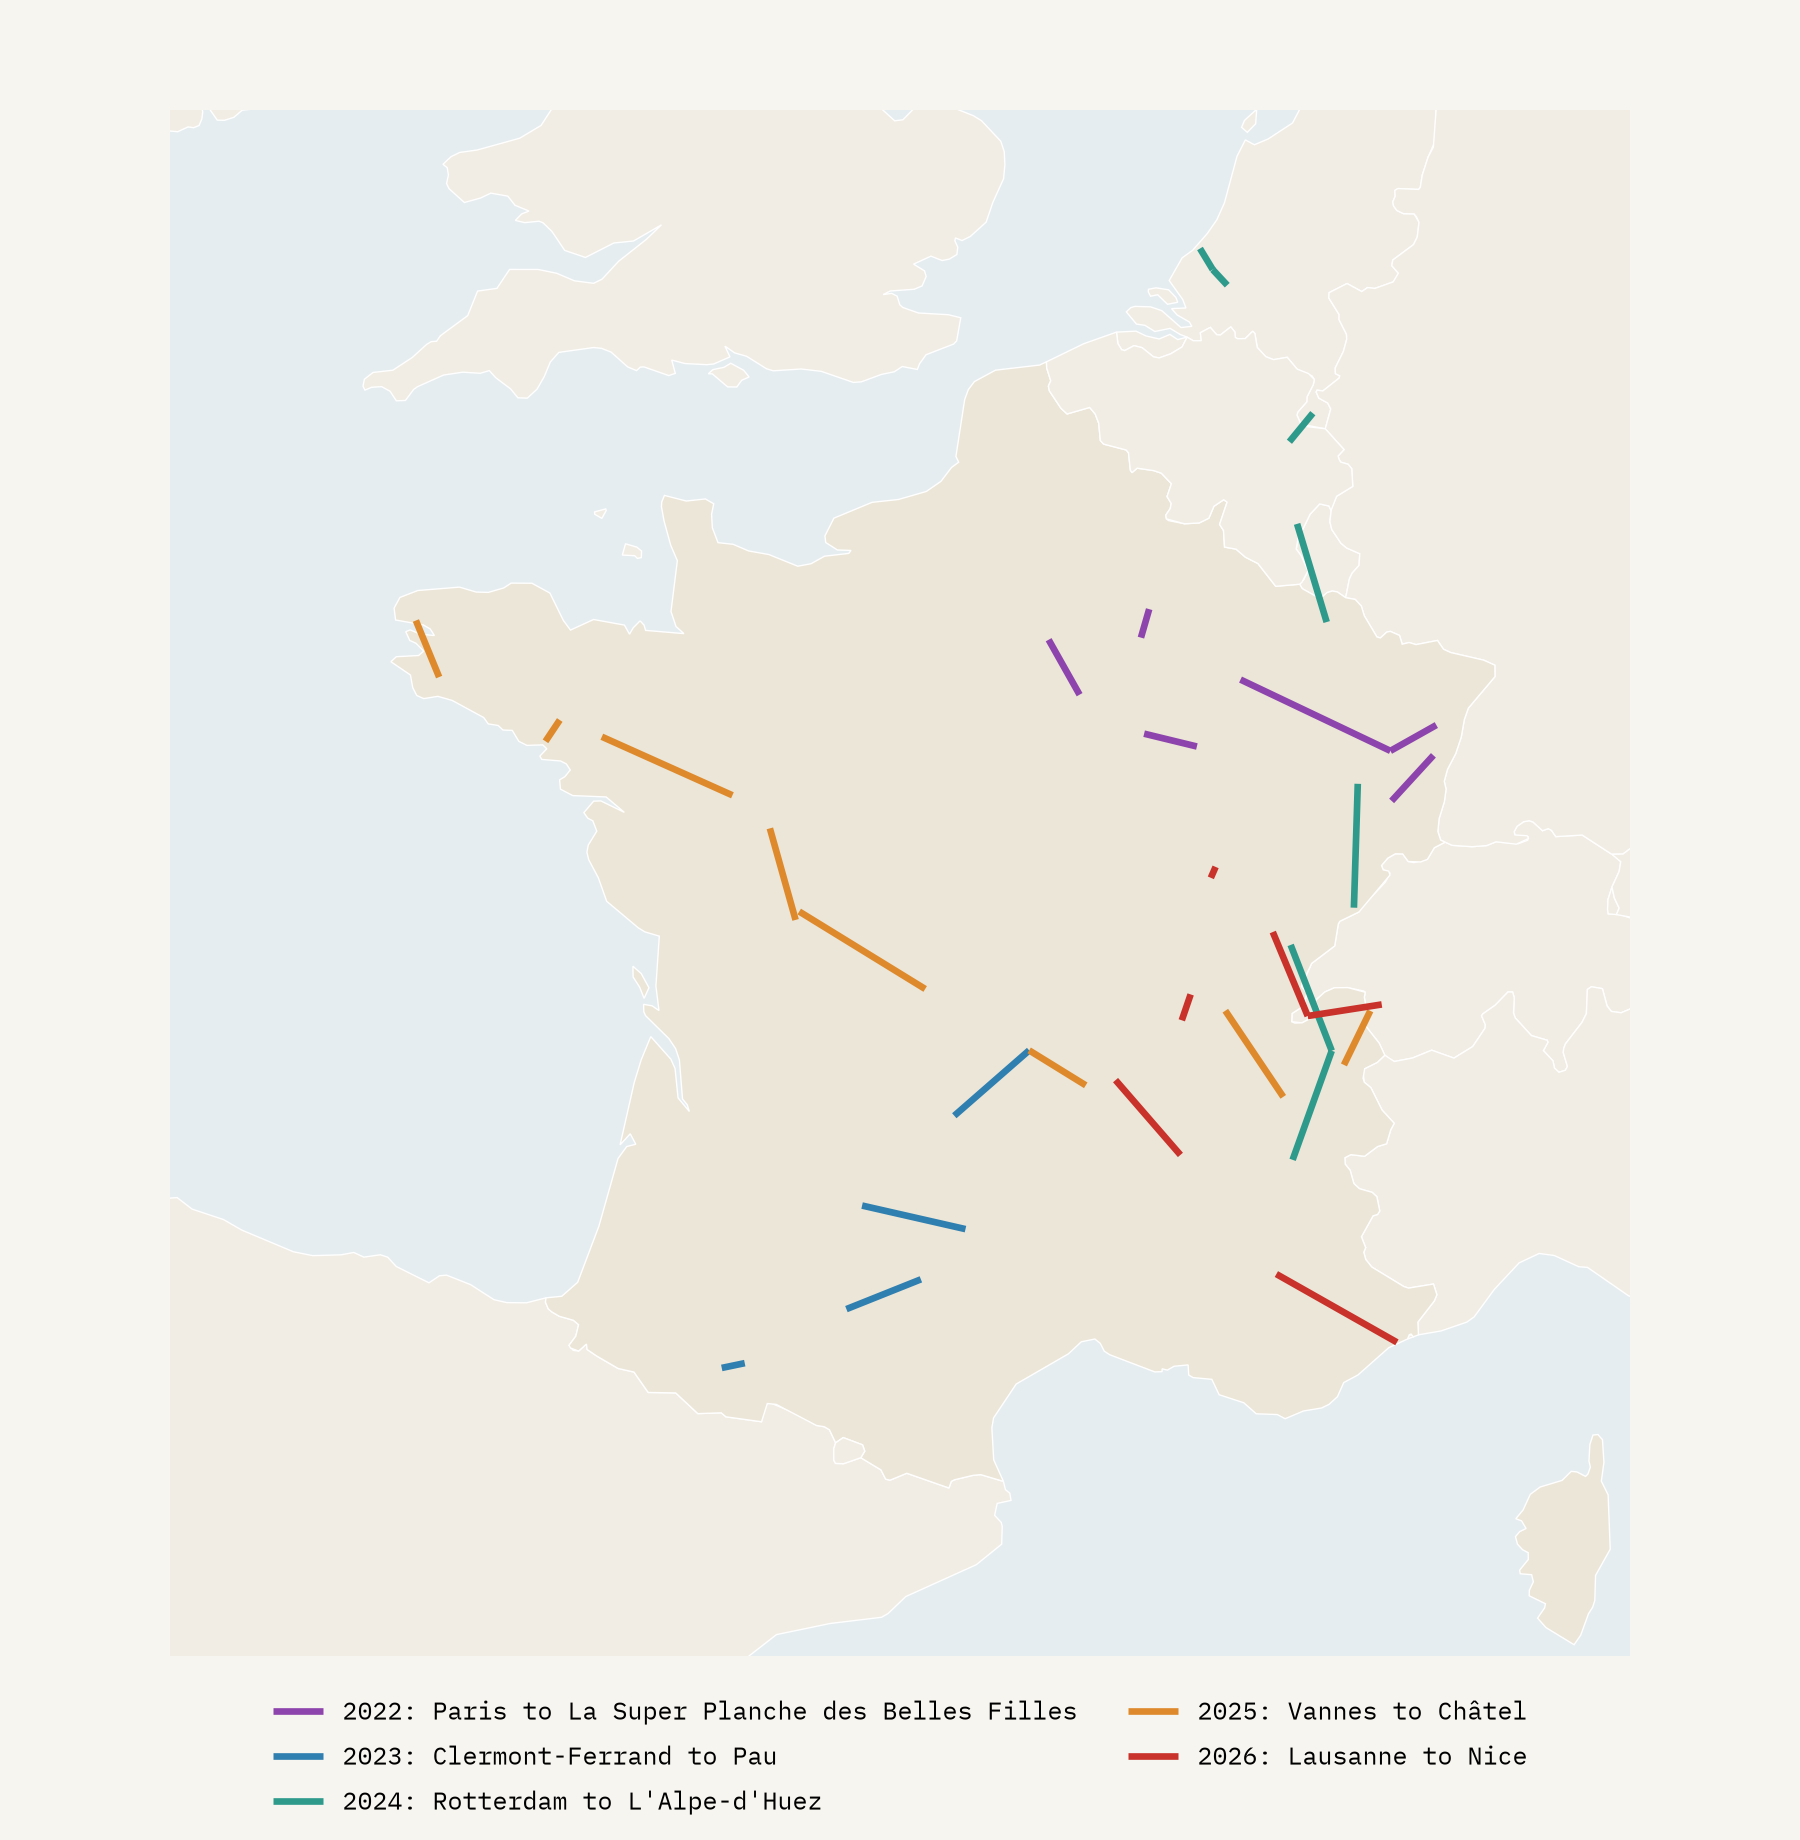
\includegraphics[width=.75\textwidth]{f_women.png}
\caption{The located stages of the Tour de France Femmes, by edition.}\label{fig:women}\end{figure}

\section{Limitations}
First, the lines are straight: they show which towns a stage joined, not the road, the climbs or the distance. Second, 207 starts and finishes are not located, mostly mountain finishes, so the map under-represents the high mountains, especially since the 1970s. Third, a few matches rest on judgement: ski stations named after a village, venues placed in their commune, and ambiguous names settled by distance. All are listed in the data files. Fourth, the stage file is a compilation of official web pages and may carry their errors; I corrected none beyond the duplicated and transfer rows. Fifth, the winners' nationalities are a hand-made addition, checked against the data only for the national team years. Sixth, ``visited'' means a start or finish: the many towns and départements that stages passed through are not in the data.

\section{Conclusion}
Mapped stage by stage, the Tour de France changes from a ring to a web. For its first three decades it was a continuous lap of France's edges; after the Second World War it moved inland, began to cross borders and, from the 1970s, to leap between regions by transfer, until most stages now start somewhere other than the last finish. It has shrunk by about two fifths in length, and its fastest winner rode almost twice as fast as the winner of 1926. Through all of this the same few towns recur, Paris first, then Bordeaux, Pau and Luchon on the road to the Pyrenees, and the race has, at one time or another, stopped in every département of the mainland.

\section*{Data and code availability}
The interactive map is at \url{https://maps.tristanhotham.com/tour-de-france/}. Data and code are at \url{https://github.com/Tristan-Hotham/tour-de-france} and archived with this paper at https://doi.org/10.5281/zenodo.23873013. Derived data and text are released under CC BY 4.0 and code under the MIT licence. Stage and rider data: LeTourDataSet by Thomas Camminady (MIT licence). Places: GeoNames (CC BY 4.0).

\section*{AI statement}
I wrote the text, with drafting and editing assistance from Claude (Anthropic), which also helped prepare the analysis code. I reviewed and checked all text and results.

\begin{thebibliography}{9}
\bibitem[Camminady(2026)]{ltd} Camminady, T. (2026) LeTourDataSet: every cyclist and stage of the Tour de France in four CSV files (commit c377920). MIT licence. \url{https://github.com/thomascamminady/LeTourDataSet}
\bibitem[A.S.O.(2026)]{letour} Amaury Sport Organisation (2026) Tour de France and Tour de France Femmes historical results. \url{https://www.letour.fr}
\bibitem[GeoNames(2026)]{geonames} GeoNames (2026) cities1000, packaged by lutangar/cities.json (commit e5e759c). CC BY 4.0. \url{https://www.geonames.org/}
\bibitem[Natural Earth(2026)]{naturalearth} Natural Earth (2026) Admin 0 countries (1:50m, 1:10m) and admin 1 states and provinces (1:10m). Public domain. \url{https://www.naturalearthdata.com/}
\end{thebibliography}
\end{document}
